\documentclass{jot}

\usepackage{makeidx}  % allows for indexgeneration
% \usepackage[pdftex]{graphicx} % PNGs
% \usepackage{amsmath, amssymb} % algebra
\usepackage[english]{babel} % deutsch
\usepackage[utf8x]{inputenc}
\usepackage[T1]{fontenc}

\usepackage{caption}
\usepackage{hyperref}
\usepackage{subcaption}

\usepackage{microtype} % optional, for aesthetics
\usepackage{tabularx} % nice to have
\usepackage{booktabs} % necessary for style
\usepackage{listings} % for sourcecode

%DIF PREAMBLE EXTENSION ADDED BY LATEXDIFF
%DIF UNDERLINE PREAMBLE %DIF PREAMBLE
\RequirePackage[normalem]{ulem} %DIF PREAMBLE
\RequirePackage{color}\definecolor{RED}{rgb}{1,0,0}\definecolor{BLUE}{rgb}{0,0,1} %DIF PREAMBLE
\providecommand{\DIFadd}[1]{{\protect\color{blue}\uwave{#1}}} %DIF PREAMBLE
\providecommand{\DIFdel}[1]{{\protect\color{red}\sout{#1}}}                      %DIF PREAMBLE
%DIF SAFE PREAMBLE %DIF PREAMBLE
\providecommand{\DIFaddbegin}{} %DIF PREAMBLE
\providecommand{\DIFaddend}{} %DIF PREAMBLE
\providecommand{\DIFdelbegin}{} %DIF PREAMBLE
\providecommand{\DIFdelend}{} %DIF PREAMBLE
%DIF FLOATSAFE PREAMBLE %DIF PREAMBLE
\providecommand{\DIFaddFL}[1]{\DIFadd{#1}} %DIF PREAMBLE
\providecommand{\DIFdelFL}[1]{\DIFdel{#1}} %DIF PREAMBLE
\providecommand{\DIFaddbeginFL}{} %DIF PREAMBLE
\providecommand{\DIFaddendFL}{} %DIF PREAMBLE
\providecommand{\DIFdelbeginFL}{} %DIF PREAMBLE
\providecommand{\DIFdelendFL}{} %DIF PREAMBLE
%DIF END PREAMBLE EXTENSION ADDED BY LATEXDIFF

% Command to generate a different version of the text for the JOT
% paper and the tech report.  The first argument is the text for the
% JOT paper, the second is for the tec report.
\newcommand\articleORtr[2]{#1}

\newcommand\hairspace{\ifmmode\mskip1mu\else\kern0.08em\fi}
\RequirePackage{xspace}

\usepackage{array} % tables
\usepackage{afterpage} % figures
\usepackage{float} % figures
\usepackage{paralist} % figures
\usepackage[shortcuts]{extdash} % figures
\usepackage{todonotes}
\usepackage{lmodern}
\lstset{%
  language=ruby,%
  basicstyle=\scriptsize,%\ttfamily,
  frame=single,%
  emph={always, once, constructor},%
  emphstyle=\bfseries,%
  % breaklines=true,
  breakatwhitespace=false,%
  literate={<<}{\tiny{$\ll$}~}{1}%
  {.?}{\bfseries\emph{.?}}{1}%
  {visible?}{visible?}{1},%
  showstringspaces=false,%
  columns=flexible}
\lstnewenvironment{code}[1][]%
{\vskip0em\noindent
  \minipage{\linewidth}
  \vspace{0.5\baselineskip}
  \lstset{%
    language=ruby,%
    basicstyle=\scriptsize,%\ttfamily,
    frame=single,%
    emph={always, once, constructor},%
    emphstyle=\bfseries,%
    % breaklines=true,
    breakatwhitespace=false,%
    literate={<<}{\tiny{$\ll$}~}{1}%
             {.?}{\bfseries\emph{.?}}{1}%
             {:x}{:x}{1}%
             {:y}{:y}{1}%
             {:high}{:high}{1}%
             {:low}{:low}{1}%
             {visible?}{visible?}{1},%
    showstringspaces=false,%
    columns=flexible,#1}}
{\endminipage\vskip0em}

\restylefloat{figure}

\usepackage{glossaries}
\newcommand{\ac}[1]{\gls{#1}}
\newcommand{\acp}[1]{\glspl{#1}}

% Acronyms
\newacronym{api}{\textsc{api}}{application programming interface}
\newacronym{cip}{\textsc{cip}}{constraint imperative programming}
\newacronym{ocp}{\textsc{ocp}}{object constraint programming}
\newacronym{oo}{\textsc{oo}}{object-oriented}
\newacronym{dsl}{\textsc{dsl}}{domain specific language}
\newacronym{frp}{\textsc{frp}}{functional reactive programming}
\newacronym{vm}{\textsc{vm}}{virtual machine}
\newacronym{jit}{\textsc{jit}}{just-in-time}

\newcommand{\eg}{e.\hairspace{}g.,\xspace}
\newcommand{\Eg}{E.\hairspace{}g.,\xspace}
\newcommand{\Ie}{I.\hairspace{}e.,\xspace}
\newcommand{\ie}{i.\hairspace{}e.,\xspace}
\newcommand{\cf}[1]{cf.\,{#1}\xspace}
% \newcommand{\todo}[1]{\framebox{\textsc{todo} #1}}

\newcommand{\zthree}{Z3\xspace}
\newcommand{\langname}{\textsc{Babelsberg}\xspace}
\newcommand{\toolname}{\textsc{Babelsberg/R}\xspace}

\newcommand{\load}{\textsc{load}\xspace}
\newcommand{\store}{\textsc{store}\xspace}

\def\sectionautorefname{Section}
\def\subsectionautorefname{Section}
\def\subsubsectionautorefname{Section}
\def\tableautorefname{Table}
\def\figureautorefname{Figure}

\title{Babelsberg: Specifying and Solving Constraints on Object Behavior}

% \subtitle{Modular Object-Constraint Programming with \Large{\langname}}
\runningtitle{Specifying and Solving Constraints on Object Behavior}

\author[affiliation=hpi/cdg, nowrap, photo=tim.png] {Tim Felgentreff} {is
  a PhD student at the Hasso-Plattner- Institute, University of
  Potsdam. His research interests are in programming languages and
  virtual machine design. Contact him at
  \email{tim.felgentreff@hpi.uni-potsdam.de}. See also
  \url{http://www.hpi.uni-potsdam.de/hirschfeld/people/felgentreff}.}
\author[affiliation=uw/cdg, nowrap, photo=alan.png] {Alan Borning} {is a
  faculty member in the Department of Computer Science \& Engineering
  at the University of Washington, at the rank of Professor since
  1993, and an Associate at Viewpoints Research Institute.  His
  research interests are in human-computer interaction and designing
  for human values, and in object-oriented and constraint based
  programming languages.  He received a BA in
  mathematics from Reed College in 1971, and a PhD in computer science
  from Stanford University in 1979. Awards include a Fulbright Senior
  Scholar Award for lecturing and research in Australia, and being
  named a Fellow of the Association for Computing Machinery in 2001.
  Contact him at \email{borning@cs.washington.edu}.}
\author[affiliation=hpi/cdg, nowrap, photo=robert.png] {Robert Hirschfeld}
{is a Professor of Computer Science at the Hasso-Plattner-Institute at
  the University of Potsdam. There he founded and leads the Software
  Architecture Group which is concerned with fundamental elements and
  structures of software, methods, and tools for improving the
  comprehension and design of complex and interesting systems. He
  received a Ph.D. in Computer Science from the Technical University
  of Ilmenau, Germany. Contact him at
  \email{hirschfeld@hpi. uni-potsdam.de}. See also
  \url{http://www.swa.hpi.uni-potsdam.de/}.}

\affiliation{hpi}{Hasso Plattner Institute, University of Potsdam}
\affiliation{uw}{University of Washington}
\affiliation{cdg}{Communications Design Group, SAP Labs}

\runningauthor{Tim Felgentreff, Alan Borning, Robert Hirschfeld}

\jotdetails{
  volume=V,
  number=N,
  articleno=M,
  year=2013,
  doisuffix=jot.2013.VV.N.aN
}

\begin{document}
\begin{abstract}
  Constraints allow developers to specify desired properties of
  systems in a number of domains, and have those properties be
  maintained automatically.  This results in compact, declarative
  code, avoiding scattered code to check and imperatively re-satisfy
  invariants.  Despite these advantages, constraint programming is not
  yet widespread, with imperative programming still the norm.

  There is a long history of research on integrating
  constraint programming with the imperative
  paradigm. However, this integration typically does not unify the
  constructs for encapsulation and abstraction from both
  paradigms. This impedes re-use of modules, as client code written in
  one paradigm can only use modules written to support that
  paradigm. Modules require redundant definitions if they are to be
  used in both paradigms.

  We present a language -- \langname~-- that unifies the constructs
  for encapsulation and abstraction
  by using only object-oriented method definitions
  for both declarative and imperative code. Our prototype --
  \toolname~-- is an extension to Ruby, and continues to support
  Ruby's object-oriented semantics.  It allows
  programmers to add constraints to existing Ruby programs in
  incremental steps by placing them on the results of normal
  object-oriented message sends.  It is implemented by modifying
  a state-of-the-art Ruby virtual machine.  The performance of 
  \DIFdelbegin \DIFdel{standard
  object-oriented }\DIFdelend \DIFaddbegin \DIFadd{Ruby }\DIFaddend code without constraints is only modestly impacted,
  with typically less than 10\% overhead compared with the unmodified
  virtual machine. Furthermore, our architecture for adding multiple
  constraint solvers allows \langname to deal with constraints in a
  variety of domains.

  We argue that our approach provides a useful step toward making
  constraint solving a useful tool for object-oriented programmers.
  We also provide example applications, written in our Ruby-based
  implementation, which use constraints in a variety of application
  domains, including interactive graphics, circuit simulations, data
  streaming with both hard and soft constraints on performance, and
  configuration file management.

  % We present an approach and extension to an object-oriented language
  % to solve constraints on the results of message sends. These
  % constraints are predicates that are continuously maintained by the
  % system.

  % Constraints are written as anonymous functions that contain
  % constraint expressions. To maintain a constraint, our approach
  % chooses a constraint solver based on the return types of the
  % messages sent in the dynamic extent of the expression execution.
  % Solvers can be flexibly bound to types such as reals or strings, but
  % also complex objects such as files or methods. Furthermore,
  % constraint solvers are implemented in application code, so
  % programmers can add domain specific solvers for their use cases.

  % Our system solves constraints by modifying objects that determine
  % the results of messages sent during the constraint expression
  % execution. Whenever imperative code changes these objects, the
  % appropriate solvers are triggered to maintain the constraints.

  % Our approach is superior to existing approaches because it relies on
  % object-oriented message sends instead of paths between objects or
  % special constraint method definitions. This property ensures both
  % encapsulation and supports the uniform access principle. This, in
  % turn, allows programmers to change the implementation of objects
  % without breaking constraint code, as well as applying groups of
  % constraints to different objects that implement the same
  % interface. Since programmers can extend the available solvers, they
  % can choose the solver that gives the best results or provides the
  % best performance to their specific application.

  % We argue that using our approach, constraint solving becomes a
  % generic tool that is not limited to specific domains. Using a
  % Ruby-based implementation, we show example applications that apply
  % constraints to interesting new domains such as performance
  % assurances and configuration file handling.

\end{abstract}

%%% Local Variables: 
%%% mode: latex
%%% TeX-master: "babelsberg_jot"
%%% End: 


\keywords{Constraints, Object Constraint Programming}

\section{Introduction}
\label{sec:introduction}
Constraints and constraint programming occur in a variety of
application domains within computer science and related fields,
including graphics, CAD/CAM, planning and operations research,
artificial intelligence, user interface toolkits, and programming
languages. A \emph{constraint} is simply a relation that
should hold.  Some examples of constraints from a variety of
application domains are: that there be a minimum of 10 pixels
horizontal space between two buttons on a screen, that a resistor in
an electrical circuit simulation obey Ohm's Law, that a maximum of 10
parts per hour can be produced by a machine in a factory, that all of
the digits in a row or column or subregion of a Sudoku puzzle must be
different, that the height of a bar in a bar chart correspond to a
value produced by a simulation,
or that a streamed video play smoothly in the presence of
changing CPU and network load.  Constraints are declarative: they
specify \emph{what} should be the case rather than \emph{how} to
achieve it.  They thus provide flexibility in the way they can be
employed, since a single constraint can typically be used in multiple
ways.

A number of features are desirable in constraint programming to solve
a useful set of problems.  Unfortunately it is in general much easier
to state constraint problems than to solve them --- some problems are
extremely difficult, and others are undecidable. On the other hand,
for some restricted but very useful classes of constraints, quite
efficient solvers are available.  Therefore, practical solvers impose
restrictions on the kinds of constraints they can solve, for example,
by supporting only floats and not integers or requiring numeric
equalities and inequalities to be linear.  For example, the Cassowary
solver \cite{badros-tochi-2001} can solve multi-way constraints on
floats; Z3 \cite{de2008z3} can do the same for reals, integers, and
booleans; Kodkod \cite{torlak2007kodkod}, Z3, and Ilog
\DIFdelbegin \DIFdel{\mbox{%DIFAUXCMD
\cite{puget1994c++}
}%DIFAUXCMD
}\DIFdelend \DIFaddbegin \DIFadd{\mbox{%DIFAUXCMD
\cite{puget1994c++,ilogmanual}
}%DIFAUXCMD
}\DIFaddend can enumerate solutions; and DeltaBlue
\cite{freeman-benson-phoenix-1989} can solve multi-way constraints
using local propagation.  An even more restricted approach is to only
consider one-way constraints that can compute an output value given
new inputs, but not vice versa
(\eg \cite{hudson-uist-1996,myers-ieee-computer-1990}).

Thus, in general a variety of solvers are
needed, depending on the type domain and particular characteristics of
the constraints.  It is also useful to have these solvers interoperate
to find a solution to a particular problem. Furthermore, in some
application domains, it is important to support soft as well as hard
constraints, that is, constraints that should be satisfied if possible
as well as constraints that must be satisfied. Finally, in the presence of
frequent changes, incremental solvers are required that can efficiently
re-solve a set of constraints as input values are changed or
constraints added and deleted.  Interactive graphical systems provide
examples of all of these: they include constraints on complex objects
such as points and rectangles as well as floats and integers, soft
constraints to express preferences regarding \DIFdelbegin \DIFdel{the }\DIFdelend layout, and require
incremental solvers to efficiently re-solve constraints repeatedly\DIFdelbegin \DIFdel{as
}\DIFdelend \DIFaddbegin \DIFadd{,
for example when }\DIFaddend a part of the figure is moved.

In this work, we focus on \DIFdelbegin \DIFdel{highly dynamic }\DIFdelend constraints over objects and primitive types
such as floats, integers, and booleans (\eg for interactive graphical
applications) \DIFdelbegin \DIFdel{and system invariantsto support
writing resilient and self-healing systems , but not constraints for
search or enumerating }\DIFdelend \DIFaddbegin \DIFadd{that can describe system invariants, for example to
write systems that adhere to a specification, as well as highly
dynamic constraints that can be created, added, modified, and removed
at run-time. In contrast, this work does not support constraints for
searching or enumerating multiple }\DIFaddend solutions to a constraint model.

There are two main alternatives for incorporating constraints into
imperative programs. The most common way is via a constraint solver
library.  This has the advantage that no changes are required to the
underlying programming language, but \DIFdelbegin \DIFdel{has }\DIFdelend the disadvantage that \DIFdelbegin \DIFdel{, besides writing
the constraints, }\DIFdelend the solver
needs to be invoked explicitly at appropriate times during the
execution. If it is not, the programmer may inadvertently ignore or
bypass the constraints.  An alternate technique is to support
constraints directly in the underlying programming language.  This
addresses the problem of inadvertently bypassing the constraint
system, because the programming language ensures that the solver is
invoked whenever neccessary. This approach also typically provides a
more convenient syntax for writing constraints, either using a
separate \ac{dsl} \DIFdelbegin \DIFdel{embedded in }\DIFdelend \DIFaddbegin \DIFadd{in conjunction with }\DIFaddend the host language (with the
drawback of having to learn essentially two programming languages), or
(as in the work reported here) by allowing constraints to be written
in the host language itself.  In both cases there is the cost of
having to support a new or extended programming language.

Prior approaches of the latter kind typically provide a unified
runtime, a semantics for the interactions between declarative and
imperative code, and a linguistic symbiosis. As an extension of these,
this work additionally unifies the programming constructs for
encapsulation and abstraction by using only object-oriented methods,
classes, and inheritance for defining behavior and structure in both
the imperative and declarative paradigm.

We present our design for integrating constraints with a dynamic,
object-oriented language that preserves a familiar imperative
programming model, called \langname, and describe an implementation of
that design as an extension to Ruby~\cite{flanagan2008ruby}, called
\toolname. Key contributions for \langname with respect to language
design are as follows.

\begin{itemize}
\item The semantic model for \langname is a direct extension of an
  object-oriented model with dynamic typing, object encapsulation,
  classes and instances or prototypes with methods, and message sends.
  It supports placing constraints on the results of message sends
  rather than just on object attributes --- thus, we argue, being more
  compatible with object-oriented encapsulation and abstraction than
  prior approaches in \ac{cip}. \DIFaddbegin \DIFadd{The only restrictions are: a) an
  expression that is used as a constraint must evaluate to a boolean
  (the constraint is that it evaluate to true); b) the expression should
  return the same result on repeated evaluation (so that, for example, a
  random number generator would not qualify); and c) variables used
  in the expression must be used in single assignment fashion.
}\DIFaddend \item The syntax of \langname is a strict superset of that of the base
  language \DIFdelbegin \DIFdel{-- }\DIFdelend \DIFaddbegin \DIFadd{--- }\DIFaddend with only one minor extension to allow a question-mark
  as method name \DIFdelbegin \DIFdel{-- }\DIFdelend \DIFaddbegin \DIFadd{--- }\DIFaddend making it easy for the programmer to write and
  read constraints and object-oriented code.
\item \langname includes meta-level facilities that allow libraries to
  construct soft as well as hard constraints, and constraints that
  support incremental solving.
\end{itemize}

Additional contributions with respect to implementation techniques are
as follows.

\begin{itemize}
\item We present a technique for implementing object constraint
  languages, which uses a primitive to switch the interpreter between
  imperative evaluation, constraint construction, and constraint
  solving modes.  In imperative evaluation mode, the interpreter
  operates in the standard fashion, except that \load and \store
  operations on variables check for constraints, and if present,
  obtain the variable's value from the
  constraint solver or send the new value to the solver (which may
  trigger a cascade of other changes to satisfy the constraints).  In
  constraint construction mode, the expression that defines the
  constraint is evaluated, not for its value, but rather to build up a
  network of primitive constraints that represent the constraint being
  added.  The interpreter keeps track of dependencies in the process,
  so that, as needed, the solver can be activated or the code to
  construct the constraint can be re-evaluated.
\item \langname provides an architecture \DIFdelbegin \DIFdel{for constraint solvers }\DIFdelend that supports multiple
  constraint solvers, which makes it straightforward to add new
  solvers, and \DIFdelbegin \DIFdel{that }\DIFdelend \DIFaddbegin \DIFadd{which }\DIFaddend does not privilege the solvers provided with the
  basic implementation (they are simply the solvers that are in the
  initial library).
\item We describe a working prototype system, integrated with a state
  of the art Ruby virtual machine and \ac{jit} compiler. In the
  absence of constraints, the performance of a program written in the
  host language (Ruby) is only modestly impacted.
\end{itemize}

\toolname is a general-purpose object constraint language, and we have
implemented a variety of example programs, including a video streaming
example with both hard and soft constraints on performance,
interactive graphical layout examples (which exercise soft constraints
and incrementality), electrical circuit simulations, and solvers for
puzzles such as Eight Queens and cryptarithmetic.

The rest of this paper is structured as
follows. \autoref{sec:related-work} presents an overview of related
work in constraint programming. \autoref{sec:soft-constraint-theory}
provides the theoretical background for constraint priorities and
incremental solving. In \autoref{sec:object-constraint-programming},
we present the features of \langname; how these features are
implemented is described in
\autoref{sec:implementation}. \autoref{sec:evaluation} presents our
performance evaluation, applications written in \toolname, and a
comparison of \langname's features with related
approaches. \autoref{sec:conclusion} describes future work and
concludes.  \DIFaddbegin \DIFadd{A companion technical report \mbox{%DIFAUXCMD
\cite{felgentreff-babelsberg-tr}
}%DIFAUXCMD
provides additional details and sample }\langname \DIFadd{programs in an
appendix.  (The body of the technical report is the same as an earlier
draft of this article.)
}\DIFaddend 

\section{Related Work}
\label{sec:related-work}
Consider a graphical rectangle implemented as a pair of points --
origin and extent -- with a method to test whether the origin is in
the visible (\ie positive) part of the coordinate system, and a
method to calculate its area.
\begin{code}
class Rectangle
  attr_accessor :origin, :extent

  def visible?
    origin.x >= 0 and origin.y >= 0
  end

  def area
    extent.x * extent.y
  end
end%*\label{code:rectangle}*)
\end{code}

Suppose this rectangle encompasses some information that we want to
make sure remains on screen entirely. To that end, the area of the
rectangle should never be less than 100 square pixels and its origin
should remain visible. The constraints are that the
\lstinline{visible?} method always returns true, and the area method
always returns a value $\geq$ 100. (Note that the \lstinline{visible?}
method contains two inequalities to form a conjunctive constraint --
both conditions must be satisfied to satisfy the constraint.  It would
be straightforward to include two additional tests that
\lstinline{origin.x + extent.x <= DISPLAYWIDTH} and
\lstinline{origin.y + extent.y <= DISPLAYHEIGHT}; these are omitted
for simplicity.)

For imperative languages, the usual approach to dealing with such
dynamic constraints is to leave it entirely up to the programmer to
ensure that they are satisfied --- the constraints are either just in
comments and documentation, or perhaps in the form of
machine-checkable assertions.  For the latter case, programmers
typically write assertions to fail early if these constraints are
unexpectedly not satisfied~\cite{rinard2005exploring}.

Alternatively, 
in an object-oriented language like Ruby, we might ensure
that these constraints are satisfied, for example using
aspect-oriented programming \cite{kiczales1997aspect} to intercept
writes to either origin or extent (lines 9--10 in the following code) 
and execute a corrective action (lines 3--5).
\begin{code}
class RectAspect < Aspect
  def ensure_constraints(method, rect, status, *args)
    rect.origin.x = 0 if rect.origin.x < 0
    rect.origin.y = 0 if rect.origin.y < 0
    rect.extent.x = 100.0 / rect.extent.y if rect.area < 100
  end
end

RectAspect.new.wrap(Rectangle, :postAdvice, "extent=")
RectAspect.new.wrap(Rectangle, :postAdvice, "origin=")
\end{code}

However, the above code has a number of problems:
\begin{itemize}
\item The constraints are expressed in a form that makes them
  non-obvious --- the branch conditions have to be carefully checked to
  ensure they catch all undesired states, and the reader has to infer
  the constraint from the conditions (for example, that the checks for
  non-negativeness express the visibility constraint.)
\item All modifications that may invalidate the constraints have to be
  intercepted --- if the advice is insufficient or not executed at the
  correct times, the constraints may be violated through parts of the
  execution.
\item There are multiple possible solutions to the constraints, but
  which one should be selected is not explicit in the code.  (For
  example, a rectangle with area 200 instead of 100 would also satisfy
  the minimum area constraint.)  Without a declarative specification,
  it is nontrivial to decide whether this code will find the optimal
  solution. In the presence of competing soft constraints, \ie
  multiobjective optimizations, finding a solution becomes even harder
  (as discussed in \autoref{sec:soft-constraint-theory}.)
\end{itemize}

\subsection{Constraint Solver Libraries}

To address the aforementioned problems, another approach is to use a
library that provides one or more constraint solvers that allow us to
express our constraints explicitly. There is a huge range of libraries
that can be called directly from the imperative code.  One way of
classifying them is by the \emph{type domain} of the constraints (for
example, real numbers or finite domains or arbitrary objects); whether
their solver can solve constraints in a general way or just select
from a given set of functions (\eg given $c=a+b$, can it solve for any of
$a$, $b$, or $c$, or several variables simultaneously; 
or can it only find a value for $c$ given $a$ and $b$); 
and whether the solver supports particular features, such
as incremental solving.

A few solvers of particular interest for the programming language
community are \zthree~\cite{de2008z3}, a state-of-the-art SMT solver
from Microsoft Research designed for theorem proving (\eg for program
verification), and kodkod~\cite{torlak2007kodkod} for constraints over
finite domains.  Solvers for use in interactive graphics systems
include Cassowary~\cite{badros-tochi-2001}, an incremental solver for
linear equality and inequality constraints that supports soft
constraints as well as hard ones, the \DIFdelbegin \DIFdel{Aukland }\DIFdelend \DIFaddbegin \DIFadd{Auckland }\DIFaddend Layout
Editor~\cite{lutteroth2008end}, which includes support for a GUI
builder using constraints, and earlier work on
DeltaBlue~\cite{freeman-benson-phoenix-1989}, which supports multi-way
local propagation constraints and soft constraints.  There is also a
range of commercial solvers and applications, such as the CPLEX
optimizer for mathematical programming~\cite{optimization1993using}.

For example, the following code rewrites the previous solution that
relied on state changing operations and branches, to use the \zthree
library to solve our constraints (lines 6 and 9). Additional code is
required to copy state between \DIFdelbegin \DIFdel{solver and rectangle}\DIFdelend \DIFaddbegin \DIFadd{the solver and the rectangle object}\DIFaddend .
\begin{code}
class RectAspect < Aspect
  def ensure_constraints(method, rect, status, *args)
    ctx = Z3::Context.new
    ctx << Z3::Variable.new("origin_x", rect.origin.x)
    ctx << Z3::Variable.new("origin_y", rect.origin.y)
    ctx << Z3::Constraint.new("origin_x >= 0 && origin_y >= 0")
    ctx << Z3::Variable.new("extent_x", rect.extent.x)
    ctx << Z3::Variable.new("extent_y", rect.extent.y)
    ctx << Z3::Constraint.new("extent_x * extent_y >= 100")
    ctx.solve
    rect.extent.x = ctx["extent_x"]
    rect.extent.y = ctx["extent_y"]
  end
end

RectAspect.new.wrap(Rectangle, :postAdvice, "extent=")
RectAspect.new.wrap(Rectangle, :postAdvice, "origin=")
\end{code}

Using a solver allows programmers to express constraints about the
system in terms of a solver-specific type domain (\eg reals, booleans,
uninterpreted function symbols) the solver understands. If the problem
is expressible in a type domain for which a solver is available (as
the above code is) the constraints can be written clearly.

\subsection{Domain-specific Languages for Constraints}

For specialized application domains, constraints are sometimes
available via separate \acp{dsl}. For user interface layouts, \acp{dsl}
describe relations between visible objects that can be automatically
maintained by the runtime.  Examples are
\textsc{css}~\cite{lie-css-book}, the Mac OS
X~\cite{AppleCocoaAutoLayout} layout specification language (which
uses Cassowary to solve the constraints), and the Python GUI framework
\emph{Enaml}~\cite{Enaml}. These allow programmers to express
relations such as distances between objects or parent/child
alignments. These constraints are automatically re-satisfied by the
runtime when imperative code changes the user interface.

The following is an example of an \emph{Enaml} specification for our
problem:
\begin{code}[language=python]
enameldef Main(Window):
    Container:
        constraints = [
            # the rectangle area is called contents in enamel
            contents_top >= 0, contents_left >= 0,
            (contents_bottom - contents_top) *
              (contents_right - contents_left) >= 100
        ]
\end{code}

\DIFdelbegin %DIFDELCMD < \ac{dsl} %%%
\DIFdelend \DIFaddbegin \acp{dsl} \DIFaddend allow programmers to use constraints in specific application
domains without having to write boilerplate code for triggering
constraint solving. They have found widespread adoption and renewed
interest recently, in particular through the Mac OS X layout system.

\subsection{Dataflow Constraints and FRP}

Some languages have built-in support for data flow, which allows
programmers to express unidirectional constraints between objects and
their parts. Examples of such systems are
Scratch~\cite{resnick2009scratch},
LivelyKernel/Webwerkstatt~\cite{lincke2012lively}, and
KScript~\cite{ohshima2013onward}.

The following uses LivelyKernel connections to observe changes to
\texttt{origin} and \texttt{extent} in a Rectangle \texttt{rect}.  On
each change, the transformation function is executed with the current
and the previous value and returns the new value for the field.
\begin{code}[language=java]
connect(rect, "origin", rect, "origin",
        function(origin, prevOrigin) {
            if (\DIFaddbegin \DIFadd{!}\DIFaddend this.isVisible()) return prevOrigin;
            else return origin;
        })
connect(rect, "extent", rect, "extent",
        function(extent, prevExtent) {
            if (this.area() < 100) return prevExtent;
            else return extent;
        })
\end{code}

Although these systems are not constraint solvers, programmers can use
constraint solvers (in the hook function passed to
\lstinline{connect}) to calculate new values and some systems, like
KScript, already integrate a constraint solver to use in the
connection. These approaches provide one answer to the question of 
when to trigger constraint solving.

\subsection{Integrating Constraints with a Programming Language}

Another approach to supporting constraints --- and the one adopted in
the work reported here --- is to integrate constraint support with a
general purpose programming language.  Again, there is a substantial body of
prior work in this area.  

One of the earliest examples for this approach is the Constraint Logic
Programming scheme~\cite{jaffar-popl-1987}, which evolved from logic
programming. One instance, CLP($\cal R$)~\cite{jaffar-toplas-1992},
provides constraints over real numbers in Prolog. These languages are
in the logic programming family, and in their standard form have no
notion of state or state change. Another language of this kind is
Concurrent Constraint Programming~\cite{saraswat-book}.

Such languages have significant advantages, such as a clean semantics,
but they sacrifice the familiar capabilities and programming
style of the more mainstream object-oriented paradigm.  Our goal here is to
support an object-oriented, imperative programming style that
integrates constraints syntactically and semantically.

With these goals, \langname follows the work by Freeman-Benson, Lopez,
and Borning on
\ac{cip}~\cite{freeman-benson-ecoop-1992,lopez-ecoop-1994,lopez-oopsla-1994,lopez-asi-1994}
and the Kaleidoscope language. Systems related to Kaleidoscope include
Siri~\cite{horn-oopsla-1992}, Turtle~\cite{grabmuller2004turtle}, and
\textsc{Soul}~\cite{d2004seamless}. These languages provide
constraints with syntactic integration into an object-oriented
language and allow expressing constraints on all object-oriented
values in their language. However, they require separate abstractions
and method definitions for the declarative and imperative paradigm.

BackTalk~\cite{roy1997reifying} and Ilog Solver~\DIFdelbegin \DIFdel{\mbox{%DIFAUXCMD
\cite{puget1994c++}
}%DIFAUXCMD
}\DIFdelend \DIFaddbegin \DIFadd{\mbox{%DIFAUXCMD
\cite{puget1994c++,ilogmanual}
}%DIFAUXCMD
}\DIFaddend are other systems that aim to integrate a rich set of constraint
solvers with imperative languages, but without full syntactic
integration or re-using of object-oriented method definitions. Rather,
they provide a library for unified access to a wide range of solvers
to be able to express various constraints, and methods to combine
these solvers with boolean operators or
propagation.  More recently, Kaplan~\cite{koksal2012constraints} 
syntactically integrated constraints with Scala, but again, does not
allow programmers to re-use object-oriented method definitions to
express constraints, and requires objects to be wrapped as
\emph{logical variables} to use them in constraints. All three systems
allow the programmer to enumerate possible solutions to constraints, a
goal \ac{cip} languages and the work presented here do not share.

There is also a body of work that uses constraints in other ways in
general-purpose programming languages.  For example, 
in Plan B, Samimi, Aung, and
Millstein \cite{samimi-ecoop-2010} use specifications as ``reliable
alternatives'' to implementations, so that if an assertion fails, the
system can use the specification as input to a constraint solver and
continue execution.  Similarly, Demsky and Rinard~\cite{demsky2006goal}
use constraint solvers to correct a faulty program state automatically
and continue running.  (Thus, by replacing assertions with
constraints, undesirable program states can be corrected by the
runtime.)

\subsubsection*{Constraint Imperative Programming in Kaleidoscope}
Because the current work shares many of its motivations with
Kaleidoscope, it also shares important design aspects that were
developed over the iterations of the Kaleidoscope language.  At the
same time, it embodies some significant improvements over that earlier
work, in particular, by providing a simpler semantic model that uses
ordinary methods and messages, rather than requiring a separate
concept of constraint constructors.

\paragraph{Abstractions}
Kaleidoscope supported Smalltalk-like classes and instances, and in
addition, integrated constraints with the language itself. This
integration included built-in constraints over primitive objects (such
as floats) and constraints over user-defined objects, which were
provided by \emph{constraint constructors}.  For example, the
\lstinline{+} constraint for Points could be defined using a
constraint constructor \lstinline{a+b=c} that expanded into
constraints on the \lstinline{x} and \lstinline{y} instance variables
of the three points \lstinline{a}, \lstinline{b}, and \lstinline{c}.
Separately, the language also provided \ac{oo} methods.  Both constraint
constructors and \ac{oo} methods were selected using multi-method semantics.
This accommodated, for example, the case of a constraint constructor
call \lstinline{a+b=c} in which \lstinline{b} and \lstinline{c} were
known and \lstinline{a} was unknown.

Our rectangle example can be expressed using Kaleidoscope as follows:
\begin{code}
class Rectangle
  constructor area = (n: Integer)
    always: extent.x * extent.y = n
  end

  constructor visible?
    always: origin.x >= 0
    always: origin.y >= 0
  end
end

rect = Rectangle.new
always: rect.area = 100
always: rect.visible?
\end{code}

With \ac{cip} as in Kaleidoscope, programmers can express constraints
over ordinary objects if the required \emph{constraint constructors}
are added to their classes in addition to ordinary methods.

In contrast to Kaleidoscope, \langname provides a simpler semantic
model. \langname uses the \DIFdelbegin \DIFdel{an }\DIFdelend object-oriented model with ordinary
methods using \ac{oo} message dispatch, rather than special constraint
constructors and multi-methods.  The implementation includes an
integration with a state of the art virtual machine and \ac{jit}, so
that in the absence of constraints, the performance of a program
written in the host language is only modestly impacted.

\paragraph{Mutable State}
This work's treatment of mutable state and time in \langname is very
similar to the later incarnations of Kaleidoscope. The first version
of Kaleidoscope, Kaleidoscope'90~\cite{freeman-benson-iccl-1992}, used
a \emph{refinement} model, in which variables held a stream of values,
related to each other by constraints.  Variables typically had a
low-priority \emph{stay} constraint so that they retained their value
over time, \eg \mbox{$x_t = x_{t-1}?$}.  (The question mark is a
read-only annotation: the constraint solver wasn't allowed to change
the past to satisfy constraints on the present.)  There were
facilities to access both the current and previous states of a
variable.  Object identity was only an implementation issue in
Kaleidoscope'90, and not semantically significant.
% , because a variable would never change its identity (it was a
% stream uniquely identified by its name), but only assume different
% values over time. --- may need to re-add this, if questions arise
% (Yoshiki didn't understand the sentence above without any further
% explanation
Later versions of the language (\eg Kaleidoscope'93)
\cite{lopez-ecoop-1994,lopez-oopsla-1994} switched to a
\emph{perturbation} model, in which destructive assignment can change
the state of objects (perhaps making previously satisfied constraints
unsatisfied), and the system perturbs or adjusts values to reach a new
state that best satisfies the constraints. Instead of streams of
values, a variable in Kaleidoscope'93 referred to a single object, as
in a more conventional \DIFdelbegin \DIFdel{languages}\DIFdelend \DIFaddbegin \DIFadd{language}\DIFaddend .  Kaleidoscope'93 also made object
identity a part of the language semantics, including support for
identity constraints as well as equality constraints.

%% add note about multiple cooperating solvers if implemented

% The above code states constraints clearly, and \emph{constraint
%   constructors} modularize the calculated properties visiblity and
% area so they can be used in constraint expressions.


%  However, two different
% problems arise:
% \begin{itemize}
% \item constraints can be expressed only on state which is exposed to
%   the constraint \ac{dsl}
% \item because the constraints are specified in separate languages,
%   they are hard to reason about in imperative code and it becomes easy
%   to accidentally write imperative code that will interfere with the
%   layout engine
% \item constraint \acp{dsl} such as these offer a predetermined set of
%   constraints for only a few special domain objects, so this approach
%   cannot be generalized
% \end{itemize}

% This approach, while clearly expressing the constraints, is not
% satisfactory for two reasons:
% \begin{itemize}
% \item constraints are expressed on object state, which has to be
%   copied between objects and the solver
% \item advice code is still required to capture all modifications that
%   may invalidate the constraints to trigger the solver
% \end{itemize}

% The problems with these approaches are:
% \begin{itemize}
% \item relations are uni-directional and binary, so \emph{m:n}
%   relations cannot be expressed and have to be satisfied by some other
%   mechanism
% \item connections observe state changes and trigger further state
%   changes. For the second constraint, it would be better if the
%   connection could be between the (dynamic) result of the
%   \texttt{area} method
% \end{itemize}

% However, through these constructors a two problems
% appear:
% \begin{description}
% \item[Behavior is duplicated] Developers have add \emph{constraint
%     constructors} to their objects before they can be used in
%   constraints. If they want to constrain the area and also access it in
%   from imperative code, they have to duplicate code.
% \item[Solvers are predetermined] Due to the deep integration \ac{cip}
%   languages offer only a fixed set of solvers, and are thus only
%   usable for certain domains.
% \end{description}

\section{Hard and Soft Constraints}
\label{sec:soft-constraint-theory}

As noted in the introduction, in some application domains, it is
important to support soft as well as hard constraints, that is,
constraints that should be satisfied if possible and constraints that
must be satisfied.  In \langname we use the semantics for hard and
soft constraints presented in reference
\cite{borning-lisp-symbolic-computation-1992}, which we briefly
review here.  

Informally, we consider collections of constraints, each labeled with
a \emph{priority}.  There is a distinguished priority \emph{required},
which denotes constraints that must be satisfied in any solution.
There are an arbitrary number of other priorities for soft
constraints.  The priorities are totally ordered, with higher-priority
constraints satisfied in preference to lower-priority ones.  While
both the theory and the constraint solvers that we use can accommodate
an arbitrary number of priorities, in practice programmers tend to
employ only a small number of priorities in stylized ways
\cite{badros-tochi-2001}.  In the examples in this section, we will
use the priorities \lstinline{required}, \lstinline{high},
\lstinline{medium}, and \lstinline{low}.

For example, consider the following constraints over the reals:

\begin{center}
\begin{tabular}{rl}
required &     $x+y=10$ \\
high     &     $x=8$ \\
low      &     $x=0$ \\
low      &     $y=0$
\end{tabular}
\end{center}

There is a single solution that best satisfies the constraints, namely
$\{x \mapsto 8, y \mapsto 2\}$, since this satisfies both the required
and high-priority constraints (and no other solution does so).

Soft constraints can have an associated \emph{error function} that
returns 0 iff the constraint is satisfied.  A simple error function
just returns 0 if the constraint is satisfied, and 1 if it is not; but
for reals, we often use a \emph{metric} function whose value increases
smoothly the further the variable's value is from the desired one.
For example, the metric error for a constraint $x=y$ is simply
$|x-y|$, while the error for $x \leq y$ is $x-y$ if $x$ is greater
than $y$, and otherwise 0.  For example, consider the following
constraints:

\begin{center}
\begin{tabular}{rl}
required &  $10 \leq x \leq 20$ \\
high     &  $15 \leq x$ \\
low      &  $x=5$
\end{tabular}
\end{center}

Using a metric error function, the solution is $\{x \mapsto 15\}$,
since this completely satisfies the required and high-priority
constraints, and minimizes the error for the low-priority one.

We might have two constraints with the same priority that cannot be
satisfied simultaneously:

\begin{center}
\begin{tabular}{rl}
required &     $x+y=10$ \\
medium   &     $x=0$ \\
medium   &     $y=0$
\end{tabular}
\end{center}

Reference \cite{borning-lisp-symbolic-computation-1992} describes a
number of different \emph{comparators} for specifying the desired
solution.  Two comparators of particular interest here are
\emph{locally-predicate-better} and \emph{weighted-sum-better}.
Locally-predicate-better finds a Pareto-optimal solution, that is, a
solution such that any other solution would cause a
currently-satisfied constraint with priority $p$ to be unsatisfied,
and further, that no higher-priority constraints would become
satisfied.  Weighted-sum-better finds solutions that minimize the
weighted sum of the errors for the highest-priority constraints; if
there are multiple solutions considering just the required and
highest-priority constraints, we consider the next highest priority,
and so on.  In the above example, there are two
locally-predicate-better solutions, $\{x \mapsto 0, y \mapsto 10\}$
and $\{x \mapsto 10, y \mapsto 0\}$.  If the weights on the two
medium-priority constraints are the same, there are an infinite number
of weighted-sum-better solutions, namely all $x \in [0,10], y \in
[0,10]$ such that $x+y=10$.  However, if we make the weight on say the
$x=0$ slightly higher, we get a single solution, namely $\{x \mapsto
0, y \mapsto 10\}$.

In \langname, we are interested in solvers that find \emph{a} solution
to a collection of constraints, so if there are multiple solutions,
the solver is permitted to select one arbitrarily.  (This is in
contrast to logic programming and constraint logic programming
languages, \DIFdelbegin \DIFdel{in which we want }\DIFdelend \DIFaddbegin \DIFadd{which give access to multiple or }\DIFaddend all solutions, perhaps
found by backtracking.)

Formally, a constraint is a relation over some domain $\cal D$\@.  The
domain $\cal D$ determines the constraint predicate symbols $\Pi_{\cal
  D}$ of the language, so that a constraint is an expression of the
form $p(t_{1} , \ldots , t_{n} )$ where $p$ is an $n$-ary symbol in
$\Pi_{\cal D}$ and each $t_{i}$ is a term.

A \emph{labeled constraint} is a constraint labeled with a priority,
written \mbox{$p c$}, where $p$ is a priority and $c$ is a constraint.
For clarity in writing labeled constraints, we give symbolic names to
the different priorities.  We then map each of these names onto the
integers $0 \ldots n$, where $n$ is the number of non-required
priorities.  Priority 0, with the symbolic name \lstinline{required}, is
always reserved for required constraints.

A constraint system is a multiset $H$ of labeled constraints.  Let
$H_0$ denote the required constraints in $H\!$, with their labels
removed.  In the same way, we define the sets $H_1, H_2, \ldots, H_n$
for levels $1, 2, \ldots, n$.  We also define $H_k = \emptyset$ for
$k>n$.

A \emph{solution} to a set of labeled constraints $H$ is a valuation
for the free variables in $H\!$, i.e., a function that maps the free variables
in $H$ to elements in the domain $\cal D$.  We wish to define the set $S$
of all solutions to $H\!$.  Clearly, each valuation in $S$ must be such that,
after it is applied, all the required constraints hold.  In addition, we desire
each valuation in $S$ to be such that it satisfies the non-required
constraints as well as possible, respecting their relative strengths.  To
formalize this desire, we first define the set $S_{0}$ of valuations such
that all the $H_{0}$ constraints hold.  Then, using $S_{0}$, we define the
desired set $S$ by eliminating all potential valuations that are worse than
some other potential valuation using the comparator predicate \emph{better}.
(In the definition, $c \theta$ denotes the boolean result of applying the
valuation $\theta$ to $c$, and we say that ``$c \theta$ holds'' if $c
\theta = \mbox{\bf true}$. Note that this is a specification of $S$,
not an algorithm for computing it!)
\begin{eqnarray*}
S_{0} & = &
  \left\{ \theta \mid \forall c \in H_{0} \; c \theta \mbox{ holds} \right\} \\
S & = & 
  \left\{ \theta \mid \theta \in S_{0} \wedge
       \forall \sigma \in S_{0} \; \neg \mbox{\em better\/}(\sigma, \theta,H)
       \right\}
\end{eqnarray*}

We now define the locally-predicate-better and weighted-sum-better
comparators.  As also noted above, we use an error function $e(c
\theta)$ that returns a non-negative real number indicating how nearly
constraint $c$ is satisfied for a valuation $\theta$.  This function
must have the property that $e(c \theta) = 0$ if and only if $c
\theta$ holds.  For any domain $\cal D$, we can use the trivial error
function that returns 0 if the constraint is satisfied and 1 if it is
not.  A comparator that uses this error function is a \emph{predicate}
comparator.  For a domain that is a metric space, we can use its
metric in computing the error instead of the trivial error function.
Such a comparator is a \emph{metric} comparator.

The first of the comparators, \emph{locally-better}, considers each
constraint in $H$ individually to find Pareto-optimal solutions.

{\bf Definition.}  A valuation $\theta$ is \emph{locally-better} than
another valuation $\sigma$ if, for each of the constraints through some
level $k-1$, the error after applying $\theta$ is equal to that after
applying $\sigma$, and at level $k$ the error is strictly less for at least
one constraint and less than or equal for all the rest.
\begin{eqnarray*}
\lefteqn{\mbox{\em locally-better\/} (\theta,\sigma,H) \equiv } \\
  &  \lefteqn{\exists k>0 \mbox{\rm \ \ such that}} \\
  & & \forall i \in 1 \ldots k-1 \; \forall p \in H_i \;\;
          e(p \theta) = e(p \sigma) \\
  & & \wedge \;\; \exists q \in H_k \;\; e(q \theta) < e(q \sigma)  \\
  & & \wedge \;\; \forall r \in H_k \;\; e(r \theta) \leq e(r \sigma)
\end{eqnarray*}

\emph{Locally-predicate-better} is then \emph{locally-better} using
the trivial error function that returns 0 if the constraint is
satisfied and 1 if it is not.

Next, we define a schema \emph{globally-better} for global comparators.
The schema is parameterized by a function $g$ that combines the errors
of all the constraints $H_i$ at a given level.

{\bf Definition.}  A valuation $\theta$ is \emph{globally-better} than
another valuation $\sigma$ if, for each level through some level $k-1$, the
combined errors of the constraints after applying $\theta$ is
equal to that after applying $\sigma$, and at level $k$ it is strictly less.
\begin{eqnarray*}
\lefteqn{\mbox{\em globally-better\/}(\theta,\sigma,H,g) \equiv } \\
  & \lefteqn{\exists k > 0 \mbox{\rm \ \ such that}} \\
  & & \forall i \in 1 \ldots k-1 \;\;
      g(\theta,H_i) = g(\sigma,H_i) \\
  & & \wedge \;\; g(\theta,H_k) < g(\sigma,H_k)
\end{eqnarray*}

Using \emph{globally-better}, we now define \emph{weighted-sum-better}
by selecting a particular combining function $g$.  The weight for
constraint $p$ is denoted by $w_p$.  Each weight is a positive real
number.

\begin{eqnarray*}
\mbox{\em weighted-sum-better\/}(\theta,\sigma,H)  & \equiv &
  \mbox{\em globally-better\/}(\theta,\sigma,H,g)  \\
  \mbox{\rm where\ \ } g(\tau,H_i) & \equiv & 
	\sum_{p \in H_i} w_p e(p \tau) \\
\end{eqnarray*}

Different constraint solvers find solutions for different comparators.
In our work to date, the two solvers we use that accommodate soft
constraints are DeltaBlue, which finds locally-predicate-better
solutions, and Cassowary, which finds weighted-sum-better solutions.
(When there are infinitely many solutions, as in the above example
with the two medium constraints $x=0$ and $y=0$, Cassowary has the
additional property that it finds solutions that ``tilt'' toward one
constraint or the other, so that it would \DIFaddbegin \DIFadd{find }\DIFaddend either the solution
$x=0$, $y=10$ or else $x=10$, $y=0$ --- but not for example $x=3.6$
and $y=6.4$, even though that is also a weighted-sum-better solution.)

In \langname, the comparator to be used is thus named by the choice of
constraint solver.

\subsection{Read-only Annotations}

A variable in a particular constraint (either hard or soft) can be
annotated as \emph{read-only}.  Intuitively, when choosing the best
solutions to a constraint hierarchy, constraints should not be allowed
to affect the choice of values for their read-only variables, \ie
information can flow out of the read-only variables, but not into
them.  (Alternatively we can say that constraints are only allowed to
affect the choice of values for their unannotated variables.)  For
example, consider the following constraints:
\begin{center}
\begin{tabular}{rl}
required &     $x?+5=y$ \\
medium   &     $y=20$ \\
low      &     $x=0$
\end{tabular}
\end{center}

The solution is $\{x \mapsto 0, y \mapsto 5\}$ --- the read-only
annotation on the $x$ in the required constraint prevents the solver
from satisfying the $y=20$ constraint instead of the $x=0$ one.

A \emph{one-way constraint}, as used in many solvers and systems,
including the ubiquitous spreadsheet, can be represented by annotating
all but one of the constrained variables as read-only, as in the
following example:

\begin{center}
\begin{tabular}{rl}
required &     $x?+y?=z$ \\
\end{tabular}
\end{center}

Reference \cite{borning-lisp-symbolic-computation-1992} presents a
formal, declarative specification of read-only annotations, adapted
from formalizations of read-only annotations in committed-choice logic
languages \cite{maher-iclp-1987}, but the above intuitive description
is sufficient for the current purpose.

\subsection{Support for State Change and Incrementality}
\label{sec:state-change}

When used in interactive graphical applications, as well as in other
systems involving change over time, it is important to provide the
constraint equivalent of ``frame axioms'' that specify that parts
retain their old values as the system changes; without such
constraints, we would often get counter-intuitive behavior, such as a
constrained figure collapsing to a point.  \emph{Stay constraints}
provide such a mechanism.  As far as the theory of hard and soft
constraints is concerned, a stay constraint is simply an equality
constraint $v=c$ for variable $v$ and constant $c$, typically with a
low priority.  Operationally, $c$ will be the value of $v$ at the
previous time step.

To support incrementality, we also introduce the notion of an
\emph{edit constraint}.  Formally, this again is simply an equality
constraint $v=c$ for variable $v$ and constraint $c$.  Operationally,
it is used to model \DIFdelbegin \DIFdel{rapidly }\DIFdelend changing an input value, for example in
response to the cursor position (where in this case $v$ and $c$ would
both hold points: $v$ would be a point in a diagram being moved, and
$c$ would be the cursor postion).  Edit constraints typically have a
high (but not required) priority --- the system will attempt to
accommodate the edit action, but may be prevented from doing so, for
example if a figure would leave the allowed display rectangle as a
result of attempting to move it too far.

Both DeltaBlue and Cassowary treat stay and edit constraints
specially, allowing very fast incremental re-satisfaction of a
collection of constraints as new edit values stream into the system
(and the weak stay constraints provide basic stability). Edit
constraints prepare the internal data structures of the solver for
fast resolving when specific variables change. For DeltaBlue, this
involves pre-calculating the execution plan from the edit variables.
For Cassowary, the Simplex tableau is set up so that it can be
efficiently re-optimized given new values for the edit variables.

\section{Object Constraint Programming}
\label{sec:object-constraint-programming}
\langname is an \ac{ocp} language --- the term \emph{object constraint
  programming} is chosen to emphasize the integration with widespread
object-oriented programming ideas, in particular methods, messages,
and object encapsulation.  This is in contrast to earlier work on
\ac{cip}, which emphasized separate, parallel concepts to specify and
select behavior for constraints, rather than re-using the
object-oriented behavior definitions.  Similarly, systems 
such as Kaplan, BackTalk, and Ilog Solver 
expect the objects used in constraints to be special constraint-aware
ones, rather than ordinary objects.

Our goals for \langname include a syntax that is compatible with the
base language. In our \DIFdelbegin \DIFdel{prototype }\DIFdelend \DIFaddbegin \DIFadd{initial prototype, }\DIFaddend \toolname, the base language is Ruby,
and the extensions are almost all semantic extensions, with only one
minor (and completely optional) syntactic extension. This extension
provides a more convenient syntax for writing read-only constraints. A
\DIFdelbegin \DIFdel{work-in-progress }\DIFdelend \DIFaddbegin \DIFadd{subsequent }\DIFaddend implementation of \langname in JavaScript ---
\langname/JS --- uses no syntactic extensions \DIFaddbegin \DIFadd{\mbox{%DIFAUXCMD
\cite{felgentreff-ecoop-2014}
}%DIFAUXCMD
}\DIFaddend .

The semantic model is also an extension of Ruby's, and supports all of
the existing Ruby constructs such as classes, instances, methods,
message sends, and blocks (closures). There are two semantic changes
to support constraint creation and solving.

The first semantic addition is the inclusion of the \emph{always}
primitive --- described in \autoref{sec:constr-constr-always} --- that
receives a closure, and creates a constraint from it. The constraint
is, that the last expression in the closure should return true. The
closure can reference objects, invoke methods on them, express
assertions about their identity, type, or protocol, and use
assignments and control structures. However, some restrictions apply,
and are described in \autoref{sec:constraint-restrictions}.

The second semantic addition is the provision of
\emph{constrained variables} ---
described in \autoref{sec:constrained-variables} --- whose values are
defined by a constraint solver. Constrained variables can be changed
by the solver to satisfy constraints when the system is perturbed, and
assignments to them trigger resolving with the new value. Assignments
may also fail, if that would make the constraint system unsatisfiable.

\DIFdelbegin \DIFdel{As this work is relatively recent, we offer here a }\DIFdelend \DIFaddbegin \DIFadd{In this paper we provide an }\DIFaddend English-language description of the
semantics of our constraints and the language changes\DIFdelbegin \DIFdel{, rather than a formal operational semantics (the latter is a topic of current research}\DIFdelend \DIFaddbegin \DIFadd{.  A formal
operational semantics is in preparation, with a recent
technical report \mbox{%DIFAUXCMD
\cite{felgentreff-babelsberg-formal-semantics-tr-2014}
}%DIFAUXCMD
presenting the step-by-step development of an
operational semantics for a series of versions of
Babelsberg, starting with a very simple language Babelsberg/Reals (in
which the only datatypes are real numbers along with booleans for the
constraint expressions) and through
Babelsberg/Objects (a true object-oriented language, with mutable
objects, classes, methods, messages, and inheritance, but without all the
features and idiosyncrasies of Ruby or another practical, 
widely-used language}\DIFaddend ).

\subsection{Constraints as a Language Primitive}
\label{sec:constr-constr-always}
Our first semantic extension to the basic object oriented language is
the addition of a new primitive, \lstinline{always}. This primitive
takes a closure \DIFdelbegin \DIFdel{representing the constraint}\DIFdelend \DIFaddbegin \DIFadd{argument}\DIFaddend : if the \DIFdelbegin \DIFdel{expression
}\DIFdelend \DIFaddbegin \DIFadd{last expression in the closure
}\DIFaddend evaluates to true the constraint is satisfied.  \DIFaddbegin \DIFadd{(Usually, there would
only be one expression.) }\DIFaddend The \lstinline{always} primitive evaluates
the closure using a modified interpreter\DIFdelbegin \DIFdel{that
}\DIFdelend \DIFaddbegin \DIFadd{, which }\DIFaddend collects
all objects that contribute to the \DIFdelbegin \DIFdel{expression }\DIFdelend \DIFaddbegin \DIFadd{evaluation }\DIFaddend and creates a
representation of the operations between them\DIFdelbegin \DIFdel{that a solver can use }\DIFdelend \DIFaddbegin \DIFadd{. This representation can
then be passed to a solver }\DIFaddend to satisfy the constraint. (The syntax for
\lstinline{always} is the same as for a normal method call that
accepts a closure \DIFdelbegin \DIFdel{, and is given in
}%DIFDELCMD < \autoref{sec:synt-always-prim}%%%
\DIFdelend \DIFaddbegin \DIFadd{argument}\DIFaddend .)

%DIF > % and is given in \autoref{sec:synt-always-prim}.)
%DIF > % commented out -- reference no longer works
\DIFaddbegin 

\DIFaddend As a first example, consider the following class
\lstinline{TemperatureConverter} in \DIFaddbegin \linebreak \DIFaddend \toolname, which maintains the
appropriate relation between instance variables holding Centigrade and
Fahrenheit values.

\begin{code}
class TemperatureConverter
  attr_accessor :centigrade, :fahrenheit
  def initialize
    @centigrade = @fahrenheit = 0.0
    always { centigrade * 1.8 == fahrenheit - 32.0 }
    # constraint added and solver triggered during `always'
  end
end
\end{code}

A constraint constructed through \lstinline{always} is activated
immediately. The primitive also returns a \emph{Constraint} object
that provides the interface to enable, disable, and inspect the
constraint. We assign floating-point numbers to the two fields, so
that \toolname uses a solver for floats based on their run-time
type. However, we didn't need to give them values that satisfy the
constraints --- one or both are changed to keep the constraint
satisfied.

If we make a new instance of \lstinline{TemperatureConverter} and
change either the Centigrade or Fahrenheit temperature, the other
value will be changed as well to keep the constraint satisfied:

\begin{code}
t = TemperatureConverter.new(100.0)
t.centigrade = 100.0 # triggers solver, which changes t.fahrenheit to 212.0
\end{code}

% There may be multiple constraints that together specify the desired
% solution.  For example, here are two constraint from a
% \lstinline{Resistor} class that uses Ohm's Law:

% \begin{code}
%   always { lead1.current + lead2.current == 0.0 }
%   always { lead1.voltage - lead2.voltage == resistance*lead1.current }
% \end{code}

% In combination with other constraints on the behavior of
% batteries, wires, and grounds, and Kirchhoff's Law constraints for the
% connections among them, these serve to specify the behavior of
% electrical circuits such as a Wheatstone bridge.  In this case,
% finding a solution involves solving a set of linear equations.  (See
% \autoref{sec:electrical-circuits} in the appendix
% for a listing of these classes, along with example circuits.)

In this example, the constraints are on the results of sending the
messages \lstinline{centigrade} and \lstinline{fahrenheit}. These
methods are just accessors for the corresponding fields.  However,
constraints can also include methods that perform other
computations. For example, the rectangle from
\autopageref{code:rectangle} makes available its area as a computed property
via the \lstinline{area} method.  Whether it is on screen is
computed by the \lstinline{visible?} predicate. In \toolname, we can
use these existing Ruby methods in specifying constraints on a rectangle:

\begin{code}
rect = Rectangle.new
always { rect.area >= 100 }
always { rect.visible? }
\end{code}

The first constraint says that the result returned from calling the
\lstinline{area} method should always be greater than or equal to 100,
and if, for example, another part of the program assigns to the height
of the rectangle, if necessary the width will be adjusted
automatically to keep the constraint satisfied. The \lstinline{always}
primitive discovers that the \lstinline{x} and \lstinline{y} values of
the \lstinline{extent} object are multiplied to get the result of the
\lstinline{area}, and that this result should be greater or equal to
100. This relation is passed as a constraint to a float solver.

Similarly, if a negative location is assigned to the origin, it will
be moved back to keep the rectangle visible.\footnote{There are
  multiple possible locations that satisfy the
  \lstinline{rect.visible?} constraint; here the system will move the
  origin as little as possible from the assigned location but so that
  the constraint is satisfied.  The same holds for the area
  constraint.  This behavior is a result of soft ``stay''
  constraints. These are left implicit in this example, but can also
  be stated explicitly if desired.  See Section
  \ref{sec:soft-constraint-theory}.}

By placing the constraint on the result of sending messages rather
than on fields, the system also respects object encapsulation.  The
values returned from the message sends in the rectangle example are
both primitive types (float and boolean), but they can also be
arbitrary objects.  For example, we could add a constraint on the
rectangle's center (a computed rather than a stored value, and a point
rather than a primitive type):

\begin{code}[numbers=none]
always { rect.center == Point.new(100,100) }
\end{code}

\subsubsection{Restrictions on Constraints}
\label{sec:constraint-restrictions}
When the programmer uses a method in \langname in a constraint, the
underlying implementation generates a corresponding set of (generally
simpler) constraints that can in turn be handed to an appropriate
solver.  Different language constructs in the methods can give rise to
different sets of constraints, which may be more or less difficult for
the solver.  For example, disjunctions in the method
give rise to disjunctions in the constraints sent
to the solver, and of the currently provided solvers, only \zthree
can accommodate these.

%% When the programmer uses a method in \langname in a constraint, the
%% underlying implementation generates a corresponding set of (generally
%% simpler) constraints that can in turn be handed to an appropriate
%% solver.  Different language constructs in the methods can give rise to
%% different sets of constraints, which may be more or less difficult for
%% the solver.  For example, conjunctions and disjunctions in the method
%% give rise to conjunctions and disjunctions in the constraints sent
%% to the solver, and of the currently provided solvers, only \zthree
%% can accommodate these.\todo{Check.  I thought more or less any solver
%%   could handle a conjunction.  Is this just about disjunctions? Or is
%%   it about explicit conjunctions rather than just a series of
%%   constraints?}\todo{Tim: This is about explicit conjunctions, but I'm not
%%   sure if there really is a difference to multiple separate
%%   constraints. Maybe talk only about disjunctions.}

There are however three important restrictions on constraints that
apply to all solvers.

First, evaluating the expression that defines the constraint should return a
boolean --- the constraint is that the expression evaluates to true.

Second, the constraint expression should either be free of side
effects, or if there are side effects, they should be benign,
\eg caching.  Also, repeatedly evaluating the constraint expression
should return the same thing.  (For example, an expression whose value
depended on which of two processes happened to complete first wouldn't
qualify.)  This restriction is needed to provide the correct semantics
for constraints.

Third, variables used in methods that will be called in a constraint
must be used in a \DIFdelbegin \DIFdel{single-assignment }\DIFdelend \DIFaddbegin \ac{ssa} \DIFaddend fashion.  As an example of why this
restriction is needed, consider the following method:
\begin{code}
def bad_method(x)
  sum = x
  sum = sum+2
  sum
end
\end{code}

Suppose we try to satisfy the constraint
\lstinline{10==bad_method(a)}. The system would then construct a
constraint \lstinline{sum==x} for the first line in the method, and
\lstinline{sum==sum+2} for the second\DIFdelbegin \DIFdel{(which is unsatisfiable)}\DIFdelend \DIFaddbegin \DIFadd{. This is unsatisfiable, so an
exception would be raised by the solver.
}

\DIFadd{This last restriction can be removed if methods in which variables are
multiply assigned are split into code blocks that are each
in }\ac{ssa} \DIFadd{form. Multiple assignments to the same variable are then
rewritten as assignments to distinct variables (}\eg \DIFadd{$x_t$, $x_t{+1}$,
\ldots), which are connected via equality constraints. The above
code, for example, can be split into two blocks (line 2 and lines
3-4), with the resulting constraints being  }\lstinline{sum_1==x} \DIFadd{and
}\lstinline{sum_2==sum_1+2}\DIFadd{.  Currently, this rewriting must be done by
hand by the programmer; in the future we plan to add an extension to
do this code transformation automatically}\DIFaddend .

%% \langname tracks assignments during constraints, so instead of a
%% general error, it can report if a variable is assigned multiple times
%% in a constraint.  A way to address this issue would be to treat multiply
%% assigned variables in constraints as distinct variables (\eg $x_t$,
%% $x_{t+1}$, etc.), which are connected through equality constraints,
%% similar to the original Kaleidoscope'90 refinement approach.
%% However, we believe that the additional complexity of
%% keeping track of successive versions of a variable outweighs the
%% additional expressiveness, and do not support such a feature.
%% (Note that for straight-line code it's easy to add additional variables
%% to satisfy this restriction.  Loops with such multiply assigned variables
%% need to be converted to recursions --- see the following section for
%% an example.) 
%% *** Paragraph seemed too detailed - deleted

\subsubsection{Constraints and Control Structures}
Expressions to create constraints are simply statements in the host
language, and so can appear in conditionals, loops, recursive methods,
and so forth.  Constraints themselves can also include iterations and
conditionals.  For example, here is a definition of the
\lstinline{sum} method for arrays that creates a set of addition
constraints relating the array elements and their sum, using partial
sums as intermediate variables.\footnote{The \lstinline{sum} method
  uses \lstinline{inject} (known also as \lstinline{reduce} or
  \lstinline{fold}) instead of, for example, a call to
  \lstinline{each} that repeatedly assigns to a local variable, so
  that we satisfy \langname's single assignment rule.} Similar
constructs can be used in representing more complicated structures.

\begin{code}
class Array
  def sum
    inject(0) { |partial_sum, x| partial_sum + x }
  end
end
\end{code}

% For example, the Kirchhoff's Law constraint in the
% electrical circuit examples listed in
% \autoref{sec:electrical-circuits} uses \lstinline{inject} to constrain
% the sum of the currents in $n$ connected leads to be 0.

We ship a simple local propagation solver for constraints on float
arrays. Constraints on the elements interact correctly with other
constraints on the sum and values.  For example, the programmer can
use the solver to find a value for one element, given the sum and
values for the others:

\begin{code}
a = [0.0, 0.0, 0.0]
always { a[0] == 10 }
always { a[2] == 20 }
always { a.sum == 60 }
\end{code}

This gives the solution \lstinline{a[1] = 30}.
We also have constraints on the length of an array, and the array as a
whole.  For example, for arrays \lstinline{a} and \lstinline{b}:

\begin{code}
always { a.length == 10 }
always { a == b } # == is content equality for Ruby arrays
\end{code}

%% What about the examples with cycles that won't work?  How does the
%% programmer know what will work and what won't?

\subsubsection{Constraints on Identity, Type, or Protocol}
We can also write constraints on properties of objects such as their
identity, class, and the messages that \DIFdelbegin \DIFdel{it responds }\DIFdelend \DIFaddbegin \DIFadd{they respond }\DIFaddend to.  For example:

\begin{code}
always { x is? y  } # an identity constraint
# examples of constraints on the class or message protocol of an object:
always { a.class == Point }
always { a.kind_of?(Point) }
always { a.instance_of?(Point) }
always { a.respond_to?(:theta) }
\end{code}

Identity constraints, in our current implementation, are supported
with a built-in local propagation solver. They are useful for defining
data structures (for example a circular linked list) or when modeling
aspects of the real world \cite{lopez-ecoop-1994}. For example, it is
clearly different if two train tickets are valid for the \emph{same}
or an \emph{equal} train.

For \lstinline{a.class} and \lstinline{a.instance_of?}, if
\lstinline{a} is already bound, the constraint is just a test; if it
is unbound, then the constraint could be satisfied by creating a new
instance of the appropriate class, binding it to \lstinline{a}, and
calling the \lstinline{allocate} method of the appropriate class.
Finally, \lstinline{a.kind_of?}  and \lstinline{a.respond_to?} are
only available as tests.  (One could imagine satisfying
\lstinline{a.kind_of?} by backtracking through the possible classes of
which \lstinline{a} is an instance, but this seems complicated and
without a clear use case.  The situation for \lstinline{a.respond_to?}
is similar.)

Note that a benefit of this design is that type declarations or
their equivalent are just constraints.

\subsubsection{Soft Constraints}
\label{sec:soft-constraints}
As noted in \autoref{sec:soft-constraint-theory}, soft constraints
are useful, for example, in interactive graphical
applications. Although not generally required for \ac{cip} languages,
most support soft constraints. As an example, a soft constraint
$a+b=c$, with priority \lstinline{high}, would be written in \toolname
as
\begin{code}[numbers=none]
always(priority: :high) {a+b==c}
\end{code}

In \langname, whether soft constraints can be accommodated and how
soft constraints are traded off are considered properties of the
solver. Solvers that cannot accommodate constraint priorities should
throw an exception when passed a priority. \DIFaddbegin \DIFadd{Some solvers provide means
of simulating soft constraints, for example, }\zthree \DIFadd{can produce
``unsatisfiable cores'', which is a list of constraints that cannot be
simultaneously true. Soft constraints in the list can be disabled to
try again without them. However, this provides two priorities
(required and not), and is slower, because the solver has to solve at
least twice}\footnote{\DIFadd{An upcoming version of }\zthree \DIFadd{will support soft
  constraints with arbitrary priorities and optimization directly.}}\DIFadd{.
}

\DIFaddend In our current implementation, we provide a mapping of the symbolic
priorities \lstinline{low}, \lstinline{medium}, \lstinline{high}, and
\lstinline{required}, for the Cassowary and DeltaBlue solvers.  (Our
initial experience with \toolname, and considerable prior experience
with Cassowary and DeltaBlue, imply that only a small number of
priorities are needed, and tend to be used in stylized ways
\cite{badros-tochi-2001}.)

\subsection{Constrained Variables}
\label{sec:constrained-variables}
Our other semantic extension concerns the way assignment is handled in the
\acrlong{ocp} language. In an \ac{ocp} program, variables that are
used in constraints become \emph{constrained variables}. Each variable
is determined by at most one solver, and the variable value is stored
in a solver specific data structure. Reading such variables returns
solver determined values and assigning to such variables triggers the
solver and may raise an exception, if the assignment would violate a
required constraint.

The \lstinline{always} primitive executes its closure argument using a
modified interpreter that tracks which objects contribute to the
constraint. Each variable that is accessed in the execution of the
closure is converted into a constrained variable. Then, depending on
the run-time type of the variable, the interpreter checks which of the
available solvers can solve constraints over this type, \eg Cassowary
for floats. If a suitable solver is available, the variable is
replaced with a solver-specific object that represents this variable
in the solvers' data structures. This solver object replaces the
actual value of the variable.

A solver object should respond to the subset of the interface of the
associated \ac{oo} value that its solver can solve. For example,
Cassowary can solve linear constraints over float values, so the
Cassowary variables returned for floats respond to the methods
\lstinline{+}, \lstinline{-}, \lstinline{*}, and \lstinline{/}, but
not \lstinline{sin} or \lstinline{**}. If a programmer tries to assert
a constraint using those latter methods, an exception will be raised.

Constrained variables for which no solver exists are used as constants
in the execution of the constraint expression. When these variables
change, the constraint expression has to be recalculated entirely.

Assignments to variables in constraints assert equality
constraints. This supports constructing new objects in
the predicate that connect values, but this also means that all
code blocks encountered during constraint construction must be in
single assignment form (\autoref{sec:constraint-restrictions}).

\subsubsection{Reading and Writing Constrained Variables}
When constrained variables that were replaced with solver objects are
read, their actual value is retrieved from the solver --- it is up to
the solver to convert the internal representation into a
representation suitable for the \ac{oo} language (\eg converting
reals into floats). Variables that were used in constraints, but not
replaced with solver objects, are read normally.

Assigning to a constrained variable also distinguishes these two
cases. If the variable was replaced with a solver object, instead of
storing the supplied value directly, a required equality constraint
between the variable and the new value is temporarily added to the
solver and the solver is invoked.  If the solver can satisfy the
constraints (including the new \DIFdelbegin \DIFdel{the }\DIFdelend equality), the assignment
succeeded; if not, an exception is raised.  Afterward, the equality
constraint is removed.

In the second case, the variable is used in a constraint, but no
solver is available to determine its value (\eg a string that was used
in a constraint when no string solver was available). The value of
such variables is treated as constant in the constraint. If the
variable is assigned, all constraints it participated in are disabled,
and their closures are re-executed to create new constraints. This,
too, may lead to a situation where some solvers cannot satisfy their
constraints. In that case, the old constraints are re-enabled, the
assignment is undone, and an exception is raised. \DIFaddbegin \DIFadd{Undoing the
assignment is necessary to ensure that no inconsistent system state
arises -- an assignment either works or fails completely.}
\DIFaddend 

\subsubsection{Stay Constraints}
In imperative languages, programmers expect their variables to retain
their values, unless some assignment operation changes them.
\autoref{sec:state-change} describes how constraints interact with
state change. For example, in interactive graphical applications, when
moving one part of a constrained figure, the user generally expects
other parts to remain where they are unless there is some reason for
them to change to satisfy the constraints.  A desire that something
remain the same if possible is represented as a \emph{stay
  constraint}, which may have an associated priority.  For example,
this stay constraint says that we prefer that x keep its value, if
possible, when satisfying other constraints:
\begin{code}[numbers=none]
always { x.stay(:low) }
\end{code}

For those solvers that support soft constraints, \langname
automatically adds a lowest-priority stay constraint to every
constrained variable so that it keeps its old value if possible when
satisfying the other constraints. \DIFaddbegin \DIFadd{This also directs the solver to find
a solution that is close to the prior value, if a variable does have
to change.
}\DIFaddend % \todo{What happens with solvers that don't support soft constraints?
% Is there anything that causes constrained variables to keep their
% old values?}\todo{Tim: no. Z3 tends keep values fairly stable, but
% there's nothing that keeps it from changing variables all over the
% place. programmers have to add more constraints if they want to get
% more reasonable results from Z3}

\subsubsection{Read-only Variables}
Some variables should not be modified by the solver (for example, in
an interactive application, dragged objects should follow the mouse,
not vice-versa). To express this, \langname includes support for
read-only variables as described in
\autoref{sec:soft-constraint-theory}. In \toolname, variables are
marked as read-only by sending the question mark method
({\bfseries\emph{?}}) to them in a constraint expression. Ruby does
not normally allow the question mark as a method name --- instead,
\toolname extends Ruby's syntax to support this. (Having a special
syntax for this is purely a convenience rather than being an essential
aspect of \toolname, and the JavaScript implementation of \langname
\DIFaddbegin \DIFadd{\mbox{%DIFAUXCMD
\cite{felgentreff-ecoop-2014}
}%DIFAUXCMD
}\DIFaddend uses a global function \lstinline{ro} instead.)

Read-only variables are useful, for example, for parameterized
constraints so the solver knows not to change the parameter to satisfy
the constraint:
\begin{code}
class Rectangle
  def fix_size(desiredsize)
    always { self.area == desiredsize.? }
  end
end
\end{code}

Without the annotation, a solver might
change the local variable \lstinline{desiredsize} rather than the
receiver.

% Read-only variables also play a central role in our architecture for
% cooperating constraint solvers, serving as ``gateways'' to control
% information flow among the solvers.  See
% \autoref{sec:cooperating-solvers}.

\subsubsection{Incremental Resatisfaction}
Some applications involve repeatedly re-satisfying the same set of
constraints with differing input values.  A common case is an
interactive graphical application with a constrained figure, where we
move some part of the figure with the mouse.  For such applications,
it is important to re-solve the constraints
efficiently. \autoref{sec:state-change} introduced \emph{edit
  constraints}, which prepare the internal state of a solver for rapid
re-satisfaction.
%% ELIMINATED THIS (or are we having an edit war?  did I already
%% eliminate it?  If so you can put it back)
%% For \langname, this means that only one edit can be
%% active for a given solver. To assign new values to variables other
%% than those that are being edited, the edit constraint has to be
%% removed and a new one including all the variables that are expected to
%% change has to be created.
In \toolname, edit constraints must used explicitly with a particular
solver. An \lstinline{edit} method is provided as part of the
Cassowary library, another is included with DeltaBlue.  These methods
use the meta-level \ac{api} of the \lstinline{Constraint} class to
query which variables participate in a constraint, create edit
constraints for them, and feed \DIFdelbegin \DIFdel{the stream }\DIFdelend \DIFaddbegin \DIFadd{new values }\DIFaddend into the resulting edit
variables.  Other libraries with support for incremental resolving can
provide similar methods. Users thus can take advantage of incremental
solvers when available to re-satisfy constraints very quickly.

The provided \lstinline{edit} method takes a variable to be edited, a
stream (an object that responds to \lstinline{next}) that provides the
new values, and optionally a priority.  (The priority defaults to the
highest non-required one.)  The solver then repeatedly re-solves 
the constraints given the new values for edit variables.  If the edit
constraint is required, the system
raises an exception if the constraints cannot be satisfied with the
new edit value.  Finally, when the
stream is empty, it removes the edit constraint and returns.  Note
that this works if the stream is being fed from another process that
provides new values only when available --- the process that has the
edit constraint should just block until one is available.

For example, suppose we make an instance of
\lstinline{TemperatureConverter}.  Then we can give 100 new values to
\lstinline{centigrade}, and have \lstinline{fahrenheit} change
correspondingly each time (this is useful, for example, if we combine
this with a graphical slider that a user can drag to input new
values):

\begin{code}
converter = TemperatureConverter.new
enumerator = (0..99).each
edit(enumerator) {converter.centigrade}
\end{code}

The stream need not contain only primitive types --- a common case in
interactive graphics is a stream of new point values for a location of
something being moved.  The implementation of edit constraints is
discussed in \autoref{sec:implementing-edit-constraints}.

\subsection{Solving Constraints}
\label{sec:solvers}
Given a set of constraints, we need to find a solution to them.
\langname provides an architecture that supports multiple constraint
solvers, that makes it straightforward to add new solvers, and that
doesn't privilege the solvers provided with the basic implementation.
(They are simply the solvers that are in the initial library.)  In the
current implementation of \toolname, the available solvers are
Cassowary, \zthree, a solver for float and integer arrays, and
DeltaBlue.

Currently, programmers must explicitly indicate which solvers are
available in a given program, just as they choose other libraries
appropriate for the application. Solvers register themselves for
specific types, and are then chosen eagerly based on the run-time type
of the variables that occur in \DIFdelbegin \DIFdel{the }\DIFdelend \DIFaddbegin \DIFadd{a }\DIFaddend constraint.  Only one solver can
be registered for a particular type. 

In cases where different solvers can handle the same types (for
example, both \zthree and Cassowary handle constraints on floats in
\langname/R), the programmer has to decide which solver to use by
activating only the desired one. The simplest way to do this is to
only include the desired library. There is also the option to provide
the solver as an additional argument to \lstinline{always}. In some
cases, this choice may simply be a matter of preference, however,
other restrictions apply. For example, since Cassowary cannot solve
nonlinear equations, the developer should select \zthree instead:
\begin{code}[numbers=none]
always(solver: Z3::Instance) { a ** 2.0 < 16 }
\end{code}
Developers must be aware that solvers may represent types differently
internally. For example, \zthree works on reals, but its C \ac{api}
represent results as double-precision floating point numbers, so
rounding errors may occur.
% \todo{I think we need to have some more discussion about floats
%   vs. reals.  Z3 supports reals, but don't these need to be
%   represented as floats in Babelsberg/R?  And Cassowary just works
%   with floats.}  \todo{Z3 works on reals, but its API already returns
%   them as double-precision floats, which is what Babelsberg/R uses for
%   its Float objects, too. I have mentioned this two paragraphs above,
%   but maybe that's not enough?}
% \todo{Let's leave it for now, but perhaps come back to this later.
%   The remaining question is how much the programmer needs to be aware
%   of roundoff and other numerical issues in programming with
%   constraints.  Cassowary has been pretty robust with respect to
%   roundoff.  One place I can imagine it coming up is if we use a
%   constraint as a test, and it fails due to roundoff errors.  Others???}

For opaque data structures (such as an
\textsc{SDL}\footnote{\url{http://libsdl.org/}} window), the solver
cannot set properties directly, but has to use the \DIFdelbegin \DIFdel{correct }\DIFdelend \ac{api}
instead. In that case, a local propagation solver like DeltaBlue must
be used and, besides a predicate, a list of setter \DIFdelbegin \DIFdel{functions }\DIFdelend \DIFaddbegin \DIFadd{expressions }\DIFaddend must be
provided. The following constraint will make a rectangle fill the
\textsc{SDL} window, or the window will be shrunk to fit the
rectangle.
\begin{code}
always(solver: DeltaBlue::Solver::Instance,
       priority: :high,
       predicate: {window.extent == rectangle.extent}) {[
  window.extent <-> { window.set_video_mode(rectangle.extent) },
  rectangle.extent <-> { rectangle.extent = window.get_video_mode }
]}
\end{code}

Additional arguments to \lstinline{always} are passed to and
interpreted by the solver. In this case, the \lstinline{predicate} and
\lstinline{priority} arguments are passed to DeltaBlue and not
interpreted by \langname. \DIFaddbegin \DIFadd{In the constraint closure, the list of
setters is provided by connecting the target variable and the setter
expression using the }\lstinline{<->} \DIFadd{syntax.
}\DIFaddend 

Developers might write constraints that are too difficult to solve, or
for which no solver exists. In that case, the constraint expression is
simply evaluated as a test that is checked by the runtime whenever a
variable changes that may change the result of the test. If the test
fails, an exception is raised explaining that no solver for the
constraint was available.

We are currently working on adding support for cooperating constraint
solvers, so that several solvers can work together to find a solution
to constraints that connect variables from different domains
\cite{borning-coop-solvers-2012}.
% .  See \autoref{sec:cooperating-solvers}.

\subsection{Constraint Duration and Activation}
\label{sec:constraint-durations-and-activation}
Constraints have \emph{durations} during which they are active.  
The \lstinline{always} duration declares
that its constraint becomes active when the \lstinline{always}
statement is evaluated and remains active indefinitely after that,
unless explicitly deactivated.

As mentioned in \autoref{sec:constr-constr-always}, the
\lstinline{always} primitive returns a \emph{Constraint} object that
provides meta-level access to control constraint activation,
allowing it to be subsequently deactivated and reactivated.  \langname
provides two additional methods that provide more structured
control of constraint durations.
The \lstinline{once} method activates a constraint,
satisfies, and then retracts it. This is useful to initialize a system
state to satisfy a constraint. The \lstinline{assert-during} construct
takes a closure and activates a constraint for the duration of the
evaluation of the closure.

A related issue is \emph{when} constraint satisfaction is invoked.
\langname's default behavior is that constraints are immediately
satisfied or re-satisfied whenever there is a change to one of the
constrained variables.  Sometimes this is not the desired behavior,
for example, when there is a sequence of assignments that change the
state of an object, with the object being in a temporarily
inconsistent state in the midst of the assignments.  To handle this,
\langname includes a construct to allow a sequence of assignments to
be made, with solving invoked only after all the assignments have been
made.  Ruby provides multi-assignments to store values into multiple
variables in a single statement, and this is used in \toolname to
implement this construct.  If multiple variables that have constraints
on them are assigned using multi-assignment, all values are assigned
before the solver is triggered. If any constraints cannot be
satisfied, all assignments are immediately undone\DIFaddbegin \DIFadd{, again, to ensure
that assignments either succeed or fail entirely}\DIFaddend .

\section{Implementation}
\label{sec:implementation}
The Ruby \ac{vm} we use as a basis for \toolname is
\emph{Topaz}~\cite{FelgentreffTopazWroclove2013}, an experimental
\ac{vm} built using the \emph{PyPy/RPython}
toolchain~\cite{rigo2006pypy}. \DIFdelbegin \DIFdel{This has allowed us to extend the
interpreterand use RPython 's }%DIFDELCMD < \ac{vm}%%%
\DIFdel{-generation toolchain to create a
}%DIFDELCMD < \ac{vm} %%%
\DIFdel{including }\DIFdelend \DIFaddbegin \DIFadd{While Topaz is a Ruby interpreter, the
RPython toolchain provides it with }\DIFaddend a fast \ac{jit} \DIFaddbegin \DIFadd{compiler }\DIFaddend and
garbage collector. We \DIFaddbegin \DIFadd{have extended the interpreter, and inherit the
}\ac{jit} \DIFadd{and garbage collector from RPython. In this section, we }\DIFaddend first
provide an overview of the key features of the implementation before
plunging into the details.

The Topaz Ruby \ac{vm} is written in \DIFdelbegin \DIFdel{RPython, }\DIFdelend a restricted, object-oriented
subset of Python \DIFaddbegin \DIFadd{called RPython}\DIFaddend . Topaz executes Ruby \DIFdelbegin \DIFdel{code using a }\DIFdelend \DIFaddbegin \DIFadd{by compiling Ruby
source code into bytecodes and interpreting the bytecodes. The interpreter is
written in an object oriented fashion, with each bytecode implemented
as a method of the }\DIFaddend class \lstinline{Interpreter}\DIFdelbegin \DIFdel{that uses a custom bytecode set. To
store variables, the interpreter uses }%DIFDELCMD < \lstinline{Cells} %%%
\DIFdel{--- these
objectsprovide an indirection to
store values that are referenced in
block closures}\DIFdelend \DIFaddbegin \DIFadd{. Topaz also
represents Ruby language constructs such as references and scopes as
instances of RPython classes. As an example, local variables are
represented by }\lstinline{Cell} \DIFadd{objects, which provide methods to
access and update the variable's value.  In }\toolname\DIFadd{, we leverage the
object-oriented design of Topaz to implement }\ac{ocp}\DIFaddend .

The changes we made to the Topaz \ac{vm} are two-fold.  First, we
modified the interpreter to support a \emph{constraint construction
  mode} (\cf {\autoref{sec:constraint-construction-impl}}) and a
primitive to enter this mode.  Second, we extended the cells to
support \emph{constrained variables} (\cf
{\autoref{sec:constrained-variables-impl}}) by allowing the same name
to refer to multiple objects, one an object-oriented value and the
other a \DIFdelbegin \DIFdel{solver object}\DIFdelend \DIFaddbegin \emph{\DIFadd{solver object}}\DIFaddend .  (Note that this use of the same name to refer
to multiple objects is a feature of the implementation only --- it is
not visible to the programmer.)

\subsection{Constrained Variables}
\label{sec:constrained-variables-impl}
Ruby provides five types of variables: locals, instance variables,
class variables, globals, and constants.  (While constants \DIFdelbegin \DIFdel{are
supposed to }\DIFdelend \DIFaddbegin \DIFadd{should }\DIFaddend be
assigned only once, \DIFdelbegin \DIFdel{it is not an error condition to
re-assign to a constant in Ruby}\DIFdelend \DIFaddbegin \DIFadd{this is simply a convention in Ruby, and is not
checked by the interpreter}\DIFaddend .)  Of these \DIFaddbegin \DIFadd{variable types}\DIFaddend , we allow three
as constrained variables: locals, instance variables, and class
variables.

\DIFdelbegin \DIFdel{Variables are constrained by using them }\DIFdelend \DIFaddbegin \DIFadd{Ordinary variables are converted automatically to constrained variables 
if they are used }\DIFaddend in a
constraint expression. A constraint expression is passed to the
\lstinline{always} primitive as \DIFdelbegin \DIFdel{a }\DIFdelend \DIFaddbegin \DIFadd{an ordinary }\DIFaddend block closure. \DIFdelbegin \DIFdel{Locals referenced in closures are stored in a closure
cell , to which we added a second }\DIFdelend \DIFaddbegin \DIFadd{All locals
referenced in the expression are stored as cell objects, which in
}\toolname \DIFadd{have an additional }\DIFaddend field to store solver objects. \DIFdelbegin \DIFdel{To
speed up access to instance }\DIFdelend \DIFaddbegin \DIFadd{Instance
}\DIFaddend and class variables \DIFdelbegin \DIFdel{, Topaz uses map
transitions}\DIFdelend \DIFaddbegin \DIFadd{in Topaz are stored in
maps}\DIFaddend ~\cite{chambers1989efficient}. For \toolname, we have \DIFdelbegin \DIFdel{added
a transition }\DIFdelend \DIFaddbegin \DIFadd{extended
these }\DIFaddend to store solver objects as well as ordinary objects\DIFdelbegin \DIFdel{in
these maps, so }\DIFdelend \DIFaddbegin \DIFadd{, so that
once the }\ac{jit} \DIFadd{has warmed up, }\DIFaddend read access to solver objects is no
slower than access to ordinary objects\DIFdelbegin \DIFdel{, once the }%DIFDELCMD < \ac{jit} %%%
\DIFdel{has warmed up}\DIFdelend .

Converting ordinary variables into constrained variables has an impact
on garbage collection.  Solver objects usually have more references
pointing to them than ordinary objects --- besides their scope and
owner (in the case of instance or class variables), solver objects are
also referenced from one or more constraints. Because solver objects
can also be implemented in the host language, this means that they may
only be garbage collected if no more active constraints refer to them.

\subsection{Execution Contexts}
\label{sec:constraint-construction-impl}

To implement the different execution modes --- \emph{imperative
  execution}, and \emph{constraint construction} --- we extended the
default interpreter, and added \lstinline{ConstraintInterpreter} as a
subclass. The \DIFdelbegin \DIFdel{ConstraintInterpreter }\DIFdelend \DIFaddbegin \lstinline{ConstraintInterpreter} \DIFaddend changes how locals,
instance \DIFdelbegin \DIFdel{variable}\DIFdelend \DIFaddbegin \DIFadd{variables}\DIFaddend , and class \DIFdelbegin \DIFdel{variable }\DIFdelend \DIFaddbegin \DIFadd{variables are }\DIFaddend accessed.

\subsubsection{Imperative Execution}
This is the normal execution mode, \DIFaddbegin \DIFadd{as }\DIFaddend implemented in the Topaz
interpreter. We have extended the \store and \load \DIFdelbegin \DIFdel{bytecodes }\DIFdelend \DIFaddbegin \DIFadd{bytecode methods }\DIFaddend with an
additional check whether a variable refers \DIFaddbegin \DIFadd{just }\DIFaddend to an ordinary object
or \DIFaddbegin \DIFadd{to }\DIFaddend a solver object \DIFaddbegin \DIFadd{as well}\DIFaddend . In the latter case, instead of reading or changing the
value of the variable, the \DIFdelbegin \emph{\DIFdel{solver object}} %DIFAUXCMD
\DIFdelend \DIFaddbegin \DIFadd{solver object }\DIFaddend for the variable
receives the messages \lstinline{value} or \lstinline{suggest_value},
respectively. As long as all constraints are satisfied, this
difference is not visible to the programmer. However, while direct,
destructive assignment to a normal variable in imperative programs
always succeeds, \lstinline{suggest_value} triggers one or more
solvers. If any solver fails to satisfy its constraints \DIFdelbegin \DIFdel{with }\DIFdelend \DIFaddbegin \DIFadd{using }\DIFaddend the new
value, an exception is raised. This exception is propagated by the
\ac{vm}, and \DIFdelbegin \DIFdel{needs to }\DIFdelend \DIFaddbegin \DIFadd{should either }\DIFaddend be handled by the programmer \DIFdelbegin \DIFdel{. The }\DIFdelend \DIFaddbegin \DIFadd{or allowed to
halt execution of the program.  If an assignment
fails in this way, the }\DIFaddend variable retains its original value.

As described in \autoref{sec:constraint-durations-and-activation}, in
\toolname, if multiple variables that have constraints on them are
assigned using multi-assignment, all values are assigned before a
solver is triggered, and all assignments are undone if an exception is
raised during solving. This way, if the exception is caught, the
program is not in violation of any constraints.

\subsubsection{Constraint Construction}
The initializer for constraint objects --- usually called through
\lstinline{always} --- activates an execution context for constraint
construction. In this mode, variable values are replaced with their
associated solver objects in \load instructions. These solver objects
are created by sending \lstinline{for_constraint} to the current
variable value. This method should return an object that
responds to \lstinline{value} and \lstinline{suggest_value}. 
The \lstinline{value} method extracts the value from a solver's
internal representation, while \lstinline{suggest_value} sends the
candidate value to a solver and requests that it re-satisfy the 
constraints.  For values that do not respond to
\lstinline{for_constraint}, a generic solver object is returned that removes 
and recalculates all constraints in which it occurs whenever its value
changes.

\store instructions in this mode create equality constraints. This is
necessary to support constructing new objects in the \DIFdelbegin \DIFdel{predicate }\DIFdelend \DIFaddbegin \DIFadd{predicates }\DIFaddend that
connect values (for example, a 2d point with x and y values that were
constructed in the constraint.) However, this also means that all code
blocks encountered during constraint construction must be in single
assignment form (\cf{\autoref{sec:constraint-restrictions}}).

To support solvers written in the host language, the \ac{vm} needs a
way to distinguish code that should be executed in this mode from code
that should not.  To support this, solvers written in the host
language should be subclasses of \lstinline{ConstraintObject}.  This
class serves as a marker to leave constraint execution mode when we
enter solver code.

\paragraph{Constraint Solving}
This mode is simply a flag that is active whenever code runs in the
dynamic extent of a method of a \lstinline{ConstraintObject}. It
prevents nested sends of \lstinline{suggest_value} from causing
recursive calls to 
the solver. This is necessary to support solvers written in
Ruby, but implies that solvers themselves cannot use constraints in
their implementation.\footnote{If we wanted to support other
  cooperating paradigms in addition to constraint-oriented
  programming, we would generalize this technique to support additional
  execution contexts.}

\subsubsection*{Constraint Construction Example}
\label{sec:constraint-construction-example}
To illustrate how our implementation supports the combination of
objects and constraints, consider the rectangle example in \langname
from \autoref{sec:object-constraint-programming}.  The code
asserts that the area of the rectangle \lstinline{rect} should always
be greater than or equal to 100. The assertion is expressed by sending the
\lstinline{area} method to \lstinline{rect}, and then sending 
the \lstinline{>=} method to the
result. The only variable named explicitly in the constraint is 
\lstinline{rect}, but there are other variables that play a role in it.

In constraint construction mode, the \lstinline{rect} variable is
replaced with a generic solver object, since the class
\lstinline{Rectangle} does not implement the method
\lstinline{for_constraint}. This placeholder \DIFdelbegin \DIFdel{object }\DIFdelend delegates the message
\lstinline{area} to the rectangle. During the execution of the
\lstinline{area} method, the points are replaced with generic solver
objects, and their x and y values (floats) are replaced with \DIFaddbegin \DIFadd{specific
}\DIFaddend solver objects (for example \DIFdelbegin \DIFdel{Cassowary or }\DIFdelend \zthree variables, \cf
{\autoref{fig:architecture}}).  In this mode, the messages to the
float values return \DIFdelbegin \DIFdel{a symbolic linear expression }\DIFdelend \DIFaddbegin \DIFadd{symbolic expressions }\DIFaddend rather than calculating the
current area of the rectangle.  \DIFdelbegin \DIFdel{This linear expression }\DIFdelend \DIFaddbegin \DIFadd{The expression representing the area
of the rectangle }\DIFaddend is then sent the
message \lstinline{>=} with 100 as its argument and returns an
inequality constraint.

\begin{figure}
  \centering
  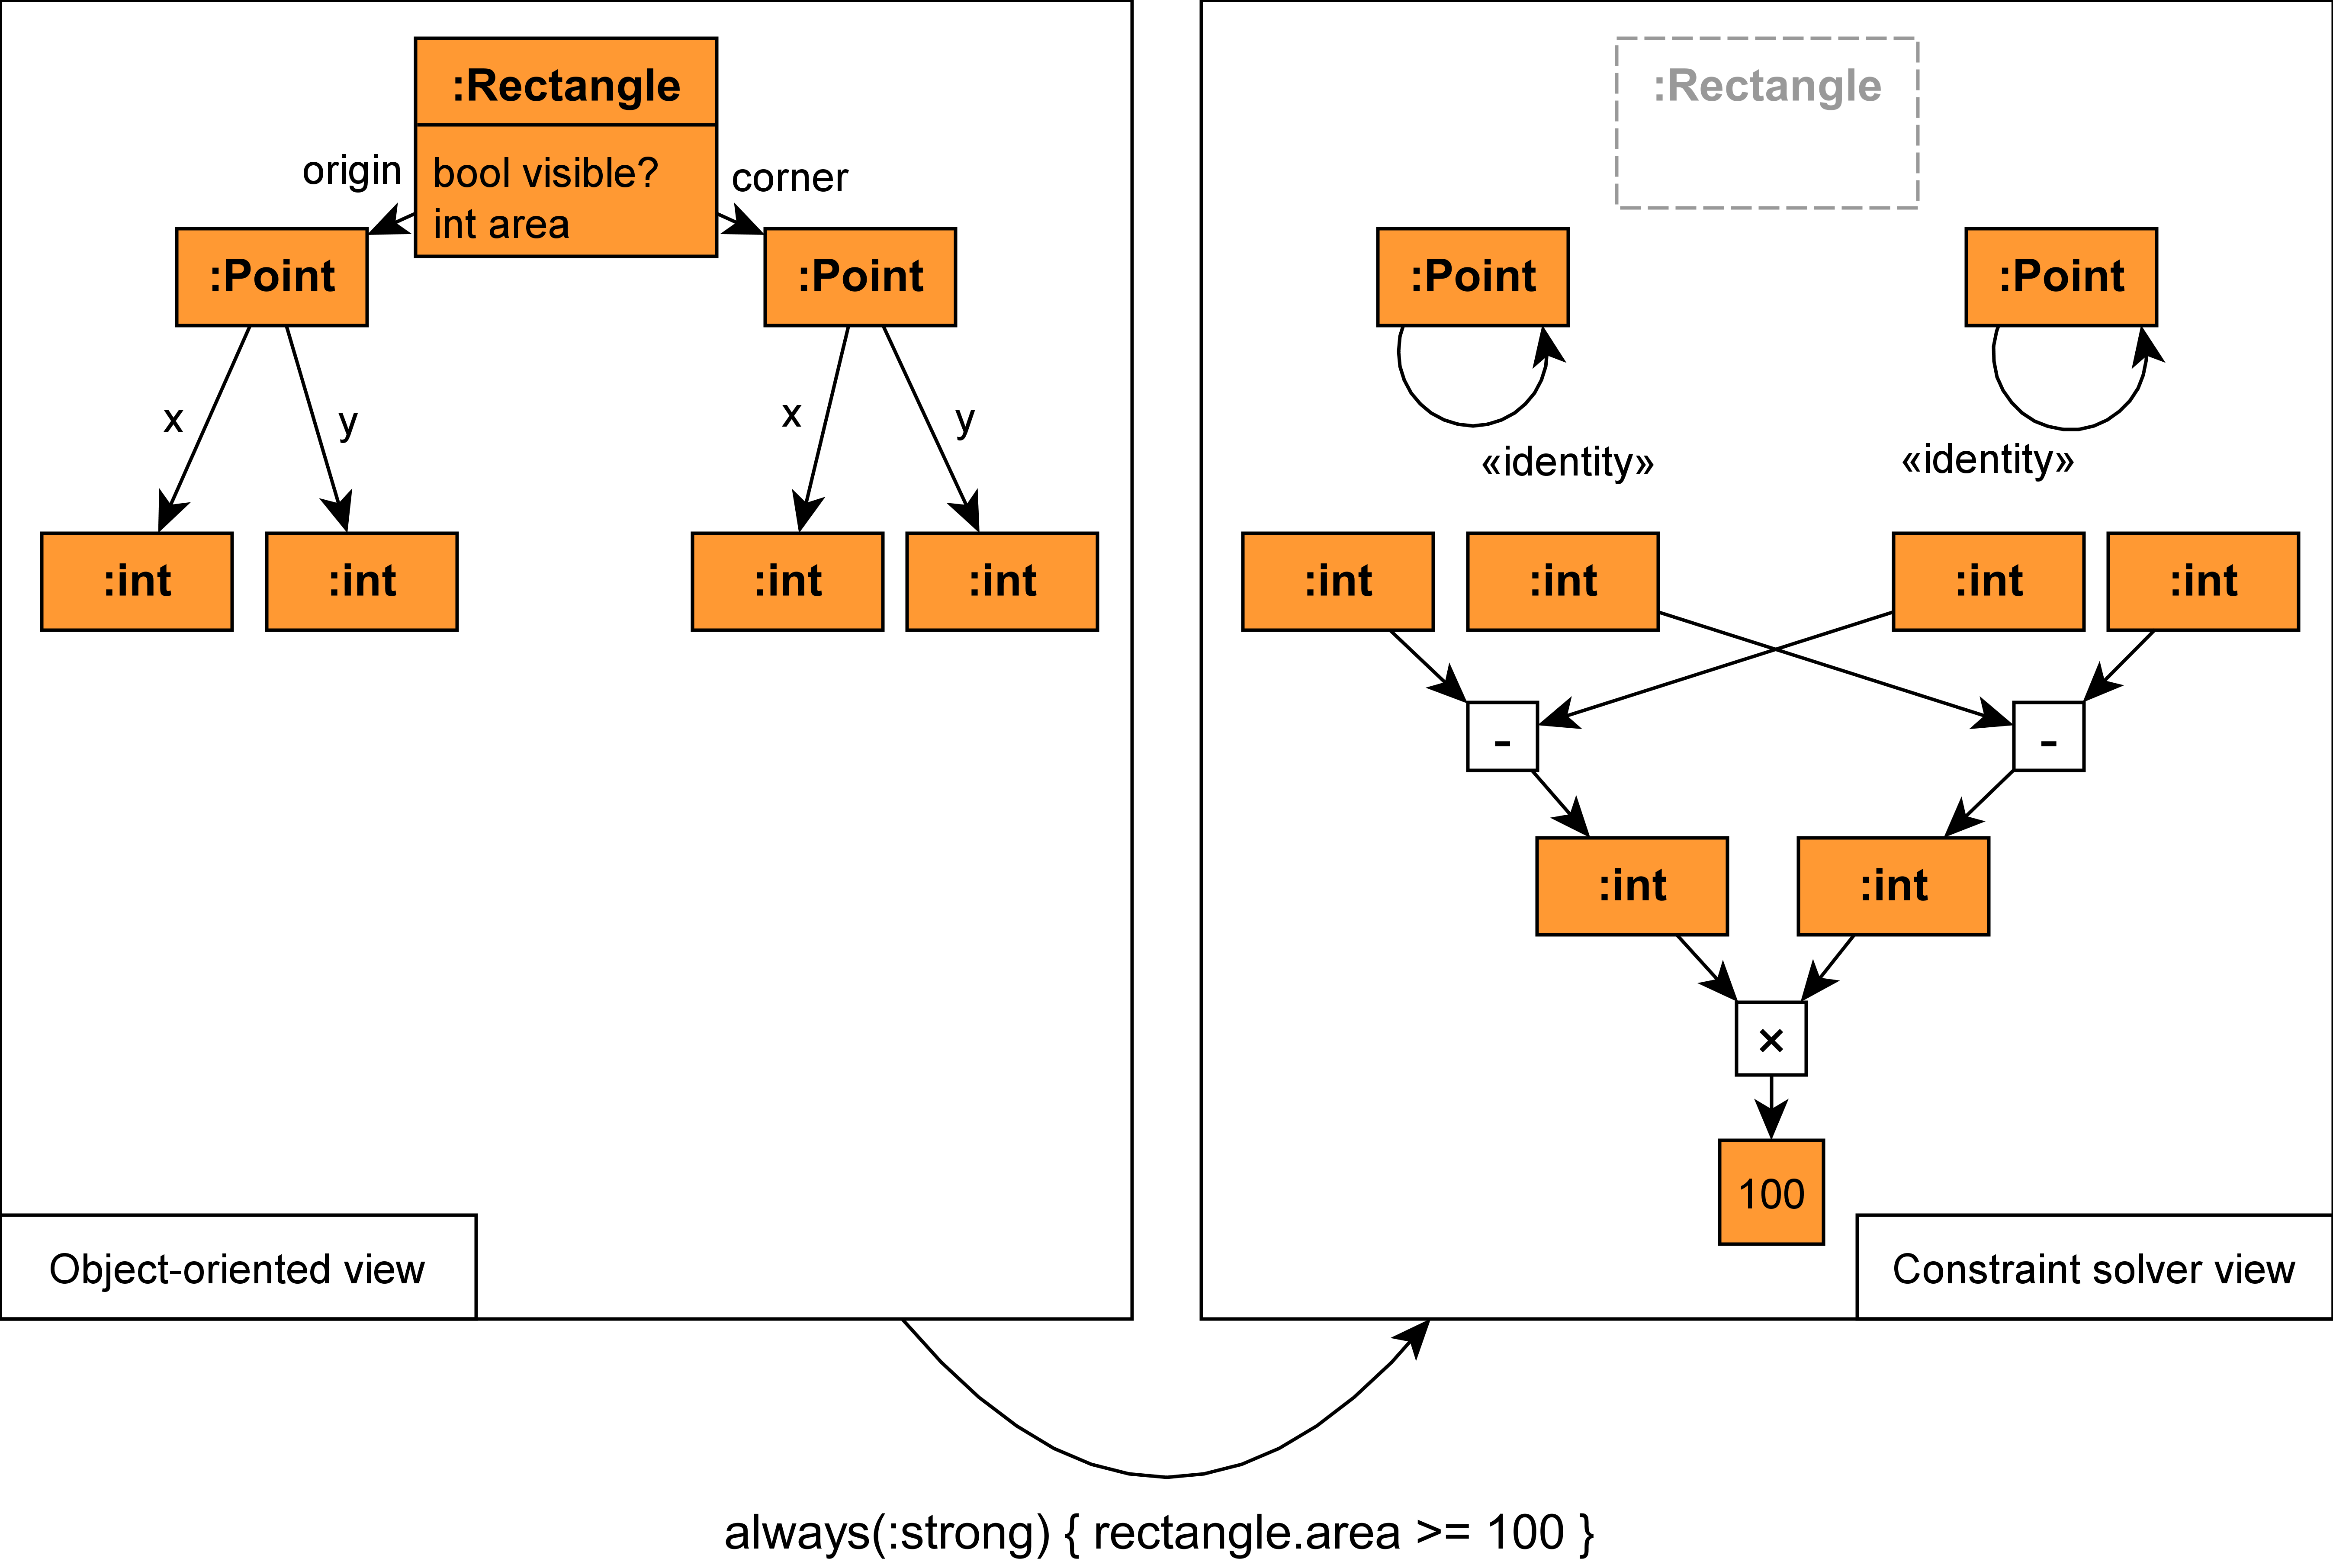
\includegraphics[width=0.98\linewidth]{architecture}
  \caption{Objects are connected through instance variables. When a
    constraint is constructed, their parts become connected through
    constraints.}
\label{fig:architecture}
\end{figure}

The constraint construction is complete when \DIFaddbegin \DIFadd{the }\DIFaddend block passed to
\lstinline{always} returns. The values and \DIFdelbegin \DIFdel{combinations thereof
created during the }\DIFdelend \DIFaddbegin \DIFadd{relations among them
produced by this symbolic }\DIFaddend execution are gathered into a
\emph{Constraint} object \DIFdelbegin \DIFdel{. It includes a) }\DIFdelend \DIFaddbegin \DIFadd{containing }\DIFaddend specific solver objects \DIFaddbegin \DIFadd{and
generic solver objects.  Specific solver objects are objects }\DIFaddend that are
connected in a \DIFdelbegin \DIFdel{constrainable way }\DIFdelend \DIFaddbegin \DIFadd{way that the solver can reason about }\DIFaddend (\eg \DIFdelbegin \DIFdel{through }\DIFdelend \DIFaddbegin \DIFadd{floats
connected via }\DIFaddend equalities or inequalities \DIFdelbegin \DIFdel{, arithmetic ,
boolean logic) and b)generic solver objects
that invalidate and
recalculate the constraint if their values change}\DIFdelend \DIFaddbegin \DIFadd{or arithmetic relations, or
booleans connected via boolean operations).  Generic solver objects
are all other objects that contribute to the constraint but about
which the solver cannot reason directly}\DIFaddend .

The constraint solvers operate on \DIFdelbegin \DIFdel{primitive constraint values }\DIFdelend \DIFaddbegin \DIFadd{specific solver objects }\DIFaddend directly to
solve the constraint. Changes made by the solver to \DIFdelbegin \DIFdel{the variables
}\DIFdelend \DIFaddbegin \DIFadd{these objects }\DIFaddend show
up in the \ac{oo} view on the next access to the variables from
imperative code, at which point \DIFdelbegin \DIFdel{the constraint }\DIFdelend \DIFaddbegin \DIFadd{their }\DIFaddend values are copied to their
\ac{oo} counterparts. Assignments to any variable encountered during
the constraint construction will trigger the solver to re-satisfy the
constraint (and potentially raise an error if the assignment is
inconsistent with the constraint).

\DIFdelbegin \DIFdel{Placeholder constraint values }\DIFdelend \DIFaddbegin \DIFadd{Generic solver objects }\DIFaddend invalidate the constraint if \DIFdelbegin \DIFdel{the }\DIFdelend \DIFaddbegin \DIFadd{their }\DIFaddend \ac{oo}
value changes through imperative assignment. This invalidation
retracts all solver objects created during constraint construction and
re-executes the block to create new solver objects and
constraints. This means that the block may be re-executed multiple
times during the run-time of the program.  (This is one reason why any
side-effects in constraints should be benign, as noted in
{\autoref{sec:constraint-restrictions}}.)

\subsection{Implementing Edit Constraints}
\label{sec:implementing-edit-constraints}
Edit constraints are used to support incremental constraint
satisfaction, and are important for achieving good performance in
interactive applications.  The \lstinline{edit} method provided as
part of \toolname's Cassowary library adds edit constraints and
repeatedly updates them with values from a stream.

Cassowary as shipped in the \toolname standard library allows the
variables and stream to hold user-defined objects as well as primitive
types. The library uses the \ac{api} of the \lstinline{Constraint}
class to access the constraint values associated with variable names,
creates edit constraints for them, and feeds the stream into the
resulting edit variables.

To use Cassowary as the solver, we need edit variables that are Floats
(\eg the x and y values of a midpoint), but we also want to do this in
an object-oriented way that respects encapsulation. To support this,
the client passes an array of method names for the return values that
should be updated in the edit constraint (\eg \lstinline{x} and
\lstinline{y} for a point --- those values may be calculated or direct
accessors.)  Cassowary creates new edit variables, and adds an
equality constraint to the return values of the methods. Thus, the
internal storage layout of the class is not visible to the programmer
from outside the object, because the
equality constraint is simply asserted on the results of message sends
using the \lstinline{always} primitive.

In the following example, the mouse locations or the mouse point might
store their x and y values directly, or might be points represented
using polar coordinates.  In either case, the edit constraints apply
to the return values of their respective \lstinline{x} and \lstinline{y}
methods:
\begin{code}[numbers=none]
edit(stream: mouse.locations.each, accessors: [:x, :y]) { mouse_point }
\end{code}

In a DeltaBlue-specific edit method, the edit constraints returned
could be simpler, since DeltaBlue local propagation methods can apply
to user-defined objects such as points, not just to floats.
The point would be simply updated rather than
dealing with its x and y coordinates separately, and the data flow
plan would update the objects constrained to be equal to the point
that represents the mouse location.

\subsection{Adding New Solvers}
\label{sec:solver-interface}
During constraint construction, the \ac{vm} sends the
\lstinline{for_constraint} message to each variable value encountered during
the execution. User code can add solvers to the system by dynamically
adding a \lstinline{for_constraint} method to those classes for which the
solver is applicable, making use of Ruby's open classes. This method
takes the name under which the variable is accessed as an argument,
and should return an object that implements a subset of the interfaces
that the solver can reason about, as well as the methods
\lstinline{value} and \lstinline{suggest_value} (as described in
\cf{\autoref{sec:constraint-construction-impl}}.)

The Cassowary solver extends the Float class:
\begin{code}
  def for_constraint(name)
    v = Cassowary::Variable.new(name: name, value: self)
    Cassowary::SimplexSolver.instance.add_stay(v)
    v
  end
\end{code}

This method creates a new variable, adds a low-priority stay so the
solver attempts to keep the value stable, and returns the constraint
object. The \ac{vm} then sends messages to this object instead of the
Float object in the context of the constraint execution.

In the case of immutable objects (such as floats and integers), the
\ac{vm} directly returns the variable value determined by the solver.
However, for mutable objects, solver libraries can provide
the method \lstinline{assign_constraint_value} to update the ordinary
object. \toolname provides a solver over numeric arrays, which uses
\lstinline{assign_constraint_value} to update the array contents. In
the \lstinline{for_constraint} method for arrays, it returns a
\lstinline{NumericArrayConstraintVariable} if all elements in the
array are instances of a subclass of \lstinline{Numeric}.
\begin{code}
class Array
  def for_constraint(name)
    if self.all? { |e| e.is_a? Numeric }
      return NumericArrayConstraintVariable.new(self)
    end
  end

  def assign_constraint_value(val)
    self.replace(val)
  end
end
\end{code}

This illustrates how the solvers provided by \toolname are simply
constraint solver libraries that extend core classes. The
\lstinline{NumericArrayConstraintVariable}, for example, allows
element access, provides the Ruby collection \ac{api} (each, map,
inject, \dots), the \lstinline{sum} method (which calculates the sum
of elements) and the message \lstinline{length}, to solve constraints
over the length of arrays.

Below is an example that asserts constraints on
\textsc{TWP}-encoded\footnote{\url{http://www.dcl.hpi.uni-potsdam.de/teaching/mds/twp3.txt}}
short strings (represented as an array of bytes). \textsc{TWP} short
strings are at most 110 bytes, with the first byte giving the length
of the string plus a tag. Line 3 constrains this particular string to
contain only capital letters (the \lstinline{?A} Ruby syntax gives the
byte value of a character).
\begin{code}
twp_str = []
always { twp_str.length == twp_str[0] + 17 }
always { twp_str.length <= 109 }
always { twp_str.each {|byte| byte >= ?A && byte <= ?Z} }
\end{code}

\section{Evaluation}
\label{sec:evaluation}

We evaluate \langname and \toolname first with respect to performance,
and second with respect to how well the language supports desirable
semantic properties for an object constraint language.

\subsection{Performance Evaluation}
\label{sec:performance-evaluation}

There are four questions we are interested in regarding performance:
a) how does constraint solving performance compare with imperative
code for satisfying constraints, b) how does \toolname performance
compare with other constraint-based languages, c) how is \DIFdelbegin \DIFdel{object-oriented
performance
}\DIFdelend \DIFaddbegin \DIFadd{performance
of pure object-oriented code }\DIFaddend affected by our extensions to the
\ac{vm}, and d) how does a practical application perform if refactored
to use constraints.

\paragraph{Constraint Solving}

\begin{figure}[b!]
    \begin{subfigure}[b]{0.48\textwidth}
      \begin{code}[basicstyle=\scriptsize,frame=none]
Iterations.times do |i|
  mouse.location_y = i
  old = mercury.top
  mercury.top = mouse.location_y
  if mercury.top > thermometer.top
    mercury.top = thermometer.top
  end
  temperature = mercury.height
  if old < mercury.top
    # moves upwards (draws over the white)
    gray.top = mercury.top
  else
    # moves downwards (draws over the gray)
    white.bottom = mercury.top
  end
  display.number = temperature
end
      \end{code}
      \caption{Imperative version}
    \end{subfigure}
    \begin{subfigure}[b]{0.52\textwidth}
      \centering
      \begin{code}[basicstyle=\scriptsize,numbers=none]
always { temperature == mercury.height }
always { white.top == thermometer.top }
always { white.bottom == mercury.top }
always { gray.top == mercury.top }
always { gray.bottom == mercury.bottom }
always { display.number == temperature }
always(:high) { mercury.top == mouse.location_y }
always { mercury.top <= thermometer.top }
always { mercury.bottom == thermometer.bottom }
always { thermometer.bottom == 0 }
always { thermometer.top == 200 }

Iterations.times do |i|
  mouse.location_y = i
end

# edit(Iterations.times) { mouse.location_y }
      \end{code}
      \caption{Object-constraint version}
    \end{subfigure}
  \caption{Interactive thermometer example from \cite{lopez-asi-1994}}
  \label{fig:thermometer-example}
\end{figure}

To answer the first question, we used an example from Kaleidoscope'93
\cite{lopez-asi-1994} and adapted it to \toolname
(\cf{\autoref{fig:thermometer-example}}).  In this example, the user
drags the upper end of the mercury in a thermometer using the
mouse. However, the mercury cannot go outside the bounds of the
thermometer, even if the user tries to drag it out. Additionally, a
gray and white rectangle on the screen should be updated to reflect
the new mercury position, and a displayed number should reflect the
integer value of the mercury top. Refactoring the imperative version
for \langname makes it more general, so the comparison is biased
towards the imperative code. However, this example demonstrates the
performance impact if an imperative program is refactored with the
goal to make it more readable, not more general.

Note that the object-constraint version may be written in two ways:
one that is more like the imperative version and assigns new mouse
locations in a loop; and a more constraint-oriented version that
declares \lstinline{mouse.location_y} as an edit variable that
triggers incrementally re-satisfying the constraints. The latter is
expected to be much faster, as Cassowary can just re-optimize a
previously optimal solution.

\autoref{fig:thermometer-benchmark} shows that the naive
object-constraint version is usually many hundreds of times slower
than the purely imperative solution. \DIFaddbegin \DIFadd{That is because the imperative
version is executing mostly machine code after a few thousand
iterations, but the constraint version has many more loops which the
}\ac{jit} \DIFadd{is struggling to optimize. }\DIFaddend Using edit constraints, repeated
solving of constraints is much faster. Keep in mind that these results
use a solver that is also written in pure Ruby, which is by itself
orders of magnitude slower than a C++ based version.

\begin{table}
  \centering
  \begin{tabular}[h]{r|c c c}
    Iterations & Imperative & Constraints & Edit Constraints \\
    \hline
    100 & 1($\sigma$0.241) & 36.1($\sigma$3.14) & 6.24($\sigma$0.828) \\
    10,000 & 1($\sigma$0.14) & 629($\sigma$6.91) & 7.72($\sigma$0.526) \\
    1,000,000 & 1($\sigma$0.12) & 45137($\sigma$458) & 52.5($\sigma$2.24) \\
  \end{tabular}
  \caption{Thermometer benchmark (normalized against imperative version)}
  \label{fig:thermometer-benchmark}    
\end{table}

\paragraph{Performance Across Different Languages}

\begin{figure}
  \centering
  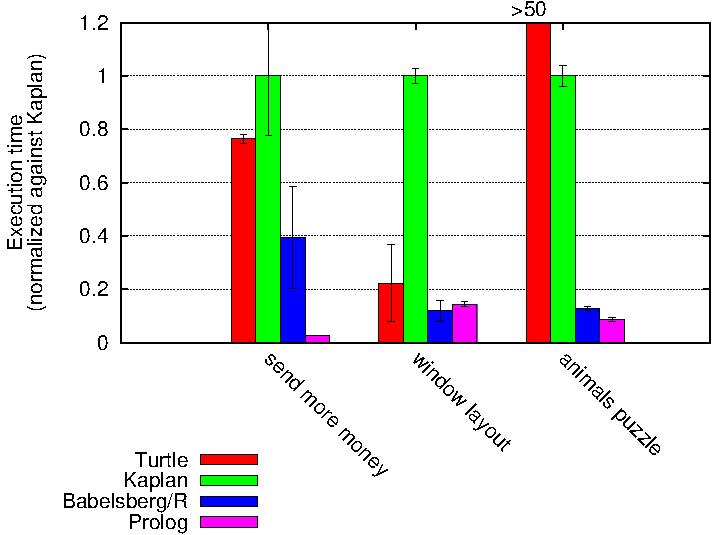
\includegraphics[width=.6\textwidth]{cip_benchmarks.pdf}
  \caption{\textsc{cip} benchmarks}
  \label{fig:cip-benchmark}    
\end{figure}

Unfortunately, good benchmarks to measure the intended usage of
languages that integrate constraints with imperative programming are
difficult to find. Papers for such languages that evaluate performance
use classical constraint solving problems. For our comparison, we
selected three such problems: the \emph{Send-More-Money}
cryptarithmetic problem
\cite{dudeney1924send}, a layout example from the Turtle
distribution (without preferential constraints), and the
\emph{Animals}\footnote{Spent \$100 to buy 100 pets. You must buy at
  least 1 of each pet. Dogs cost \$25, cats \$1, and mice
  \$0.25.} puzzle. We ran these benchmarks on Turtle, Kaplan,
and \toolname as examples of \ac{cip} languages; as well as on
SWI-Prolog's \textsc{clp} library, to compare the performance of
constraint-imperative with constraint-logic programming.

Each benchmark was run in a loop to allow the \ac{jit} in Kaplan and
\toolname to warm up, and the executions were repeated 10 times.

%% \ac{vm} in the \caption didn't work --- removed

% \begin{table}
%   \centering
%   \begin{tabular}[h]{r|c c c c}
%     Benchmark & Turtle & Kaplan & \toolname & Prolog \\
%     \hline
%     Send More Money & 2.425($\sigma$0.055) & 3.715($\sigma$0.715) &
%     1.247($\sigma$0.605) & 0.082($\sigma$0.004)\\
%     Window Layout & 0.124($\sigma$0.08) & 0.556($\sigma$0.016) &
%     0.066($\sigma$0.02) & 0.08($\sigma$0.005)\\
%     Animals Puzzle & timeout($\geq$5min) & 1.066($\sigma$0.044) &
%     0.136($\sigma$0.008) & 0.092($\sigma$0.007) \\
%   \end{tabular}
%   \caption{Constraint Benchmarks, execution times in seconds}
%   \label{fig:cip-benchmark}
% \end{table}

\autoref{fig:cip-benchmark} shows that the \ac{cip} languages are
comparable in performance, but Prolog with a constraint satisfaction
library is a better choice for these problems when no imperative
features are used. Both \toolname and Kaplan use \zthree in these
benchmarks. The difference in performance between them may be due to
the overhead of creating the constraints, but we have also found
\zthree performance to sometimes vary wildly between releases. Because
Kaplan ships an older, modified version of the Z3 library than
\toolname requires, we have not been able to compare them using the same
version of Z3.
% \todo{Alan: Can we say any more?  Is there any evidence that this probably
%   doesn't make much difference?}\todo{Tim: It probably doesn't make
%   too much difference, but that's only my guess.}

% Results after 50 runs with multitime
%% send more money
% ===> multitime results
% 1: ../turtle-1.0.0/examples/sendmory2
%             Mean        Std.Dev.    Min         Median      Max
% real        2.425       0.055       2.310       2.415       2.565
% user        2.415       0.055       2.300       2.405       2.550
% sys         0.010       0.010       0.000       0.002       0.020
% own         2.400       0.060       2.300       2.400       2.500
% ===> multitime results
% 1: ./scala-kaplan SendMoreMoney
%             Mean        Std.Dev.    Min         Median      Max
% real        4.555       0.052       4.464       4.547       4.681
% user        5.562       0.083       5.453       5.549       5.788
% sys         0.140       0.020       0.107       0.137       0.174
% own         3.715       0.715       3.035       3.225       4.840
% ===> multitime results
% 1: bin/topaz tests/constraints/constraintfixtures/smm.rb
%             Mean        Std.Dev.    Min         Median      Max
% real        1.247       0.018       1.231       1.242       1.294
% user        1.236       0.021       1.217       1.232       1.289
% sys         0.010       0.004       0.004       0.010       0.016
% own         1.200       0.605       0.490       0.965       2.045
% ===> multitime results
% 1: prolog -q --nodebug -s smm.pro -t bench(5)
%             Mean        Std.Dev.    Min         Median      Max
% real        0.082       0.004       0.076       0.083       0.088
% user        0.076       0.005       0.067       0.076       0.083
% sys         0.006       0.004       0.000       0.004       0.012
% own         0.006       0.000       0.005       0.005       0.006
%
%% turtle layouting example
% ===> multitime results
% 1: ../turtle-1.0.0/examples/layout
%             Mean        Std.Dev.    Min         Median      Max
% real        0.124       0.008       0.112       0.123       0.137
% user        0.097       0.009       0.080       0.100       0.107
% sys         0.020       0.010       0.004       0.021       0.042
% own         0.100       0.000       0.100       0.100       0.100
% ===> multitime results
% 1: ./scala-kaplan TurtleLayout
%             Mean        Std.Dev.    Min         Median      Max
% real        1.363       0.040       1.293       1.361       1.438
% user        1.810       0.038       1.730       1.814       1.855
% sys         0.080       0.018       0.053       0.078       0.122
% own         0.556       0.016       0.527       0.556       0.585
% ===> multitime results
% 1: bin/topaz tests/constraints/constraintfixtures/turtlelayout.rb
%             Mean        Std.Dev.    Min         Median      Max
% real        0.104       0.005       0.097       0.106       0.113       
% user        0.093       0.006       0.086       0.091       0.104       
% sys         0.011       0.005       0.004       0.008       0.019
% own         0.066       0.002       0.063       0.065       0.072
% ===> multitime results
% 1: prolog -q --nodebug -s layout.pro -t bench(5)
%             Mean        Std.Dev.    Min         Median      Max
% real        0.080       0.005       0.072       0.079       0.087
% user        0.073       0.004       0.067       0.073       0.082
% sys         0.006       0.004       0.000       0.006       0.012
% own         0.001       0.000       0.001       0.001       0.001
%
%% Animals puzzle
% ===> turtle didn't finish in 5 minutes
% ===> multitime results
% 1: ./scala-kaplan Animals
%             Mean        Std.Dev.    Min         Median      Max
% real        1.881       0.056       1.769       1.869       1.972       
% user        2.589       0.073       2.444       2.591       2.721       
% sys         0.106       0.013       0.087       0.106       0.131
% own         1.066       0.044       1.003       1.065       1.150
% ===> multitime results
% 1: bin/topaz tests/constraints/constraintfixtures/animal_puzzle.rb
%             Mean        Std.Dev.    Min         Median      Max
% real        0.172       0.013       0.157       0.168       0.196       
% user        0.162       0.015       0.137       0.161       0.188       
% sys         0.010       0.006       0.000       0.008       0.020
% own         0.136       0.008       0.129       0.131       0.152
% ===> multitime results
% 1: prolog -s animals.pro -t bench(5)
%             Mean        Std.Dev.    Min         Median      Max
% real        0.092       0.007       0.083       0.091       0.107
% user        0.086       0.007       0.074       0.085       0.103
% sys         0.005       0.003       0.000       0.004       0.008
% own         0.008       0.001       0.007       0.008       0.011

\paragraph{Performance of Pure Object-oriented Code}

\begin{figure}
  \centering
  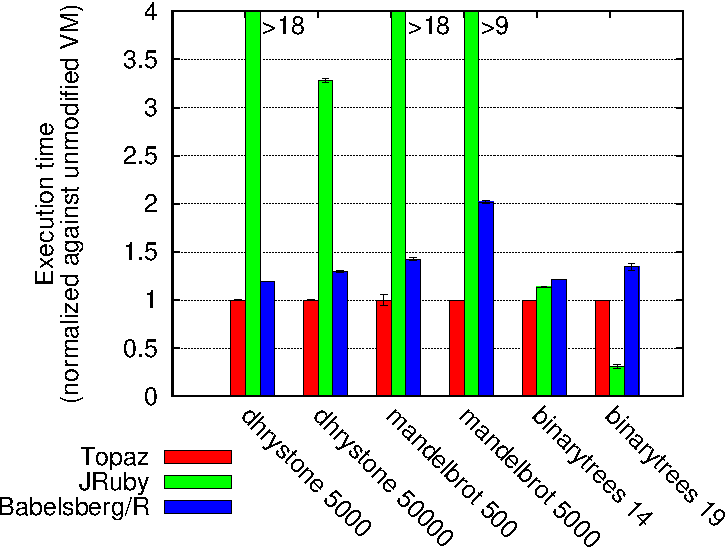
\includegraphics[width=.6\textwidth]{metatracing_vms_benchmarks.pdf}
  \caption{Metatracing \textsc{vm} benchmarks}
  \label{fig:metatracing-benchmark}    
\end{figure}

For imperative code performance, we ran a number of tests from the
metatracing \acp{vm} experiment~\cite{bolz2013impact} against the
unmodified \emph{Topaz} Ruby \ac{vm} and the \emph{JRuby} \ac{vm}.

For purely imperative code, \toolname is consistently less than 1.5
times slower in these benchmarks than the unmodified \ac{vm}
(\autoref{fig:metatracing-benchmark}). The only benchmark for which
\toolname is significantly worse than Topaz is
\emph{Binarytrees}. Binarytrees is a strongly recursive benchmark,
at which Topaz' (and thus \toolname's \ac{jit}) is bad at optimizing
(which is why JRuby does better for this benchmark). The overhead in
\toolname is due to an additional test each time a variable is
accessed, to check whether this variable participates in a
constraint. An annotation in the \ac{vm}~\cite{bolz2011runtime} allows
the \ac{jit} to remove this test when there are no constraints on
variables in the loop. The \ac{jit} consequently removes the check if
it is not needed, so all the overhead we are seeing in these results
is in code that has not been compiled by the \ac{jit}. 
Binarytrees is especially bad here, because very little code is 
compiled by the \ac{jit} for this benchmark.

Considering that JRuby and Topaz are, for these benchmarks, currently
the fastest Ruby \acp{vm}, we consider \toolname to be very performant
for purely imperative code.

\paragraph{Application Example}
We have written a simple video streaming application. This application
reads a folder with bitmaps and streams raw video to a video
player. The quality with which the video is streamed depends on a
number of variables:
\begin{description}
\item[User Preference] Users may decide not to overload their systems
  and explicitly choose a lower quality. This should be an upper
  bound for the quality of the streaming.
\item[Encoding Time] The program has only 1/25 second to encode a
  frame. If it takes longer, the quality should be automatically
  reduced to ensure smooth playback.
\item[System Load] The overall system load of the encoding system
  should be less than 80\%, to retain sufficient resources for other tasks.
\item[Quality Bounds] Whatever users choose as preferred quality, the
  quality cannot be below 0 or above 100\%.
\end{description}

In the imperative version of the application, these constraints were
explicitly checked and re-satisfied after each frame. The
object-constraint solution uses custom solvers for File contents and
method execution time.  Both versions could stream video at the
highest quality setting to up to 8 clients on an Intel i5 2.4 GHz
CPU. Both reduced the quality afterwards. Because most of the time was
spent encoding and streaming video, both versions performed
equivalently well. Most code was shared between the versions, only the
code to adjust the quality was replaced with constraints.

Both versions spent on average 43.9 ms encoding each frame and sending
it to the client. Also for both versions, 0.064 ms were spent fetching
the current load and reading the preference file. The imperative
version spent an additional 0.461 ms adjusting the quality after each
frame, whereas the object-constraint version used 2.23 ms for that. In
relation to the frame encoding time, the impact of constraint solving
was small, and the imperative code managed to encode and play 22.5
frames per second on average versus 21.6 fps for the object-constraint
code.

% \begin{figure}[h!]
%   \begin{subfigure}[b]{0.48\textwidth}
%     \begin{code}[basicstyle=\scriptsize,frame=none]
% def recalculate_quality
%   if @quality + encoding_time < 90
%     @quality = @quality + encoding_time
%   elsif @quality + encoding_time > 100 + FrameMsMax
%     @quality = 100 + FrameMsMax
%   end

%   if cpuload > 0.8 * NumberOfProcessors
%     diff = 100 * (NumberOfProcessors - cpuload)
%     if diff > 0
%       @quality -= diff
%     else
%       @quality += diff
%     end
%   end

%   if @quality > user_preference
%     @quality = user_preference
%   end
%   @quality = 0 if @quality < 0
%   @quality = 100 if @quality > 100
% end
%     \end{code}
%     \caption{Imperative version}
%   \end{subfigure}
%   \begin{subfigure}[b]{0.52\textwidth}
%     \centering
%     \begin{code}[basicstyle=\scriptsize,frame=none]
% always { @quality >= 0 }
% always { @quality <= 100 }
% always { @quality <= user_preference }
% always(:high) { @quality == user_preference }
% always { @quality + cpuload * 100 <=
%              100 + 80 * NumberOfProcessors }
% always(:high) { @quality + encoding_time >= 90 }
% always { @quality + encoding_time <=
%              100 + FrameMsMax }
%     \end{code}
%     \caption{Object-constraint version}
%   \end{subfigure}
%   \caption{Quality constraints in video streaming}
%   \label{fig:video-streaming-example}
% \end{figure}

%% \ac{vm} in the \paragraph{....} title didn't work --- changed to
%% just use capitals

\paragraph{VM Hooks for Customizing Constraint Construction}
This benchmark also demonstrates how the 
\lstinline{for_constraint} and \lstinline{assign_constraint_value} 
\ac{vm} hook methods are
useful not only for solvers, but also when programmers want to provide a
particular interpretation of certain application domain objects in
their constraints. We used this express constraints on the contents of
a preference file and the last execution time of the frame encoding
method in our constraints.

The effort to allow Cassowary to work with file content and method
execution time was small. The following class definition was enough
for us to be able to use the execution time of a method in a
constraint:
\begin{code}
class MethodTimer
  def initialize(klass, symbol)
    time = 0
    @constrained_time = Constraint.new { time }

    old_method = klass.instance_method(symbol)
    klass.define_method(symbol) do |*args, &block|
      start = Time.now
      res = old_method.bind(self).call(*args, &block)
      time = Time.now - start
      res
    end
  end

  def for_constraint(name)
    @constrained_time.?
  end
end
\end{code}

A \lstinline{MethodTimer} is instantiated with a class and the name of
a method. It wraps this method to record its execution time. When used
in a constraint, a read-only constraint object is returned that is
connected with the \lstinline{time} local variable. Because it is
read-only, the \lstinline{assign_constraint_value} method is
omitted. For the configuration file object, the
\lstinline{assign_constraint_value} method is as follows:
\begin{code}
  def assign_constraint_value(float)
    if float != @content.to_f
      raise "cannot assign to read-only file" unless @writable
      @file.truncate(0)
      @file.rewind
      @file.write(float)
    end
  end
\end{code}

This illustrates that our \ac{vm} hooks for constraint construction
provide a limited local propagation mechanism to interpret complex
objects in the type domain of a particular solver.

\subsection{Comparison with other approaches}
\label{sec:comparison}

\begin{table}[b!]
  \centering
  \begin{tabular}{l|c|c|c|c|c}
    & Libraries & \textsc{dsl} & Dataflow/\textsc{frp} & \textsc{cip} & \textsc{ocp} \\
    Unified Language Constructs & & & & & x \\
    Automatic Solving & & x & x & x & x \\
    Linguistic Symbiosis & & & x & x & x \\
    Extensible Solvers & x & & (x) & (x) & x \\
    Suitably Expressive Constraints & x & x & & x & x \\
    Performant Pure-\ac{oo} code & x & x & x & & x \\
  \end{tabular}
  \caption{Comparison of OCP with related work}
  \label{tab:cmp-constraint-lang-approaches}
\end{table}

\langname has a number of properties that we regard as desirable for
an object-constraint programming
language. \autoref{tab:cmp-constraint-lang-approaches} shows these
properties and compares \ac{ocp} to related approaches presented in
\autoref{sec:related-work}.  As a continuation of
\ac{cip}, \ac{ocp} shares most properties with \DIFdelbegin \DIFdel{the }\DIFdelend languages like
Kaleidoscope and Turtle.

\paragraph{Unified Language Constructs}
Programs in \langname appear as ordinary \ac{oo} programs if no
constraints are used, but can be easily adapted to use constraints
where it makes sense. Programmers re-use the object-oriented method
definitions to specify constraints, thus respecting object
encapsulation. Furthermore, techniques such as inheritance and dynamic
typing operate correctly with constraints.

In contrast, library and \ac{dsl} based approaches separate
constraints from imperative code through a different syntax and
semantics. For example, in languages such as Kaplan or Ilog Solver,
developers must explicitly wrap objects in classes meant for use in
constraints. \DIFdelbegin %DIFDELCMD < \ac{Frp} %%%
\DIFdelend \DIFaddbegin \Ac{frp} \DIFaddend and \ac{cip} languages use \emph{propagation
  hooks} and \emph{constraint constructors} respectively to support
constraints (propagation hooks are the functions \DIFaddbegin \DIFadd{that }\DIFaddend compute new
values for connected variables, \DIFaddbegin \DIFadd{while }\DIFaddend constraint constructors are 
\DIFdelbegin \DIFdel{the Kaleidoscopeconcept to convert }\DIFdelend \DIFaddbegin \DIFadd{Kaleidoscope's mechanism for converting }\DIFaddend constraints on user-defined objects
into primitive constraints for a solver.)

\paragraph{Automatic Solving}
Using libraries for constraint satisfaction allows programmers to
write code that (intentionally or unintentionally) circumvents
previously asserted constraints. Approaches that integrate constraints
at a language level do not allow such circumvention, and attempt to
re-satisfy constraints whenever they are violated during program
execution.

\paragraph{Linguistic Symbiosis}
D'Hondt et al.~\cite{d2004seamless} argue that linguistic symbiosis
between different programming paradigms is required to support the
evolution of programs from the object-oriented paradigm to a
constraint-oriented solution and vice versa. \ac{dsl} and library
based approaches do not support such incremental refactoring between
paradigms as well as approaches in which constraints are written in the
host language.

\paragraph{Extensible Solvers}
Libraries provide the most flexibility for choosing different solvers
depending on programmer needs. \DIFdelbegin %DIFDELCMD < \ac{frp} %%%
\DIFdelend \DIFaddbegin \Ac{frp} \DIFaddend languages can, to some extent,
be combined with solver libraries to achieve a comparable
flexibility. \ac{cip} languages also provide a more controlled way for
developers to use different solvers by writing constraint constructors
that reformulate constraints using a different solver.

In \langname, all solvers use the same interface to communicate with
the \ac{vm} so developers can add new solvers and replace existing
ones to support new type domains, or to use solvers that give better
results or performance for a particular problem.

\paragraph{Suitably Expressive Constraints}
To take advantage of the constraint paradigm, the language should
allow a rich set of constraints to be written and solved.
Multi-directional constraints are important for some applications,
while others additionally require solvers that can accommodate
simultaneous equations and inequalities.  (For example, to simulate a
Wheatstone bridge requires solving simultaneous equations, while the
video streaming example needs inequalities as well as equalities, and
both hard and soft constraints.)  On the other hand, given an overly
powerful but slow solver, it becomes all too easy to write constraints
that take a very long time indeed to solve or that are intractable.
We believe that \langname strikes an appropriate balance here, by
providing an expressive set of constraints with the solvers in the
initial library, and by allowing more powerful solvers to be added if
desired.  However, much more experience is needed to test whether in
fact this is an appropriate balance, and to adjust it as needed; and
as noted in \autoref{sec:conclusion}, an important
direction will be adding better support for debugging, explanation,
and benchmarking.

\paragraph{Performant Pure OO Code}
Kaleidoscope provided a declarative semantics for assignment, type
declaration, and subclassing. However, this declarative semantics was
also used if no actual constraints are in the program. Our
implementation approach in \toolname uses different execution contexts
for constraint construction/solving and imperative code. Combined with
a state of the art \ac{jit}, this gives performance for pure \ac{oo}
code that is generally comparable to that of a standard \ac{oo} \ac{vm}.

\section{Conclusion and Future Work}
\label{sec:conclusion}
We have presented \langname, an object constraint language that extends
an object-oriented language to support constraints, along with
an implementation as an extension to Ruby using a state of the art
virtual machine.  In contrast to other approaches, \langname unifies
the constructs for encapsulation and abstraction for both the
declarative constraint parts of the language and the traditional
imperative parts by using only object-oriented method definitions for
both declarative and imperative code.  Our implementation is
integrated with an existing object-oriented virtual machine, and
provides a standard imperative evaluation mode, a constraint
evaluation mode that accumulates constraints to send to the solver
as expressions are evaluated, and a constraint solver mode.

This work is recent and there are a number of directions for future
research.  One is to exercise the system on a wider variety of
programs, and also to work on improving the performance of the
constraint evaluation and satisfaction.  Another direction is to add
additional solvers to the library that support constraints on other
primitive storage types such as arrays, strings, and hashes, and to
implement a design for cooperating solvers.  The multi-assignment
semantics described in
\autoref{sec:constraint-durations-and-activation} provides a clean and
simple way to control when constraint satisfaction is invoked, but
experience with writing programs in \toolname is needed to decide
whether this construct is sufficiently expressive.  Yet another
direction is to introduce a ``meta-solver'' that can automatically
select one or more applicable solvers for a given set of constraints.

Another important focus will be adding better support for debugging,
explanation, and benchmarking.  (If the constraint solver is unable to
satisfy the constraints, why is this?  Or if the solver produces an
unexpected answer, how was this answer arrived at, and are there other
possible answers?  If the solver is slow, why, and are there ways to
make it faster?  Is there a more appropriate solver available?)

Our initial implementation extends Ruby, but the ideas are applicable
to other dynamic object-oriented languages, and \DIFdelbegin \DIFdel{an }\DIFdelend \DIFaddbegin \DIFadd{a second }\DIFaddend implementation in
JavaScript is \DIFdelbegin \DIFdel{also in progress}\DIFdelend \DIFaddbegin \DIFadd{now available \mbox{%DIFAUXCMD
\cite{felgentreff-ecoop-2014}
}%DIFAUXCMD
}\DIFaddend .

%%% Local Variables:
%%% mode: latex
%%% TeX-master: "babelsberg_jot_diff"
%%% End:

% In particular, a constraint extension to Javascript would be of
% particular interest given the potential for integration with Lively.

%% - solves 2 shortcoming of other constraint programming languages
%%   1. preserves encapsulation
%%   2. exchangeable solver, changeable
%%   3. modularized constraints
%% - promising approach to 1 more general problem, that we will investigate
%%   * how to integrate different execution models (declarative, imperative)
%% - good benchmark results show that it can be performant

% LocalWords:  Modularity Lugano Babelsberg hpi nowrap Felgentreff uw Borning
% LocalWords:  Hirschfeld Hasso Plattner articleno doisuffix invariants vm dsl
% LocalWords:  subregion toolkits interoperate superset incrementality resize
% LocalWords:  cryptarithmetic checkable DISPLAYWIDTH DISPLAYHEIGHT attr rect
% LocalWords:  accessor RectAspect args postAdvice dataflow SMT kodkod Aukland
% LocalWords:  DeltaBlue multi CPLEX ctx booleans runtime run-time css Enaml enameldef
% LocalWords:  FRP LivelyKernel Webwerkstatt KScript prevOrigin isVisible CLP
% LocalWords:  prevExtent Siri Samimi Aung Millstein Demsky Rinard mileaux JIT
% LocalWords:  Kaleidoscope'90 Kaleidoscope'93 TemperatureConverter fahrenheit
% LocalWords:  lead1 lead2 boolean disjunctions unsatisfiable 's parameterized
% LocalWords:  desiredsize Durations durations PyPy RPython toolchain RPython's
% LocalWords:  jit globals oo ConstraintInterpreter bytecodes initializer api
% LocalWords:  bytecode subclasses ConstraintObject unevaluated constrainable
% LocalWords:  equalities ary refactored basicstyle Metatracing i7 Ghz elsif i5
% LocalWords:  metatracing performant FrameMsMax FrameTime cpuload MethodTimer
% LocalWords:  NumberOfProcessors klass Ghz frp cip ocp Smalltalk inlines Z3 's
% LocalWords:  lookup subclassing Ghz Ghz Ghz FRAGE sind da nicht richtig drin
% LocalWords:  erwaehnen Prolog benchmarking Javascript Javascript DOIs ACKS p1
% LocalWords:  von Sternberg's acyclic SkyBlue iff CartesianPoint tex Z3Asts r1
% LocalWords:  LinearEqualities stringA stringB pt1 pt2 TwoLeadedObject r2 r3
% LocalWords:  wheatstone r4 ListCell DoublyLinkedListCell prev TODO  's 's cmp
% LocalWords:  Javascript multiobjective optimizations BackTalk impl JRuby lang
% LocalWords:  Binarytrees Topaz' D'Hondt et al versa refactoring Javascript
% LocalWords:  alldifferent


\backmatter
\vskip -1em
\bibliographystyle{alphaurl}

% \bibliography{qiqqa_jot_export,constraints,sprog}
\bibliography{babelsberg_with_dois}
\newpage
\abouttheauthors

\begin{acknowledgments}
\begin{quotation}
  \noindent I owe everything to my ``Mäuschen''.
\end{quotation}

%%% Local Variables:
%%% mode: latex
%%% TeX-master: "Felgentreff_2014_Babelsberg"
%%% End:

\end{acknowledgments}

\end{document}

%%% Local Variables: 
%%% mode: latex
%%% TeX-master: t
%%% End: 
